% Options for packages loaded elsewhere
% Options for packages loaded elsewhere
\PassOptionsToPackage{unicode}{hyperref}
\PassOptionsToPackage{hyphens}{url}
\PassOptionsToPackage{dvipsnames,svgnames,x11names}{xcolor}
%
\documentclass[
  12pt,
  oneside]{book}
\usepackage{xcolor}
\usepackage[top=30mm,bottom=30mm,left=25mm,right=20mm,headheight=15mm,footskip=33pt]{geometry}
\usepackage{amsmath,amssymb}
\setcounter{secnumdepth}{5}
\usepackage{iftex}
\ifPDFTeX
  \usepackage[T1]{fontenc}
  \usepackage[utf8]{inputenc}
  \usepackage{textcomp} % provide euro and other symbols
\else % if luatex or xetex
  \usepackage{unicode-math} % this also loads fontspec
  \defaultfontfeatures{Scale=MatchLowercase}
  \defaultfontfeatures[\rmfamily]{Ligatures=TeX,Scale=1}
\fi
\usepackage{lmodern}
\ifPDFTeX\else
  % xetex/luatex font selection
\fi
% Use upquote if available, for straight quotes in verbatim environments
\IfFileExists{upquote.sty}{\usepackage{upquote}}{}
\IfFileExists{microtype.sty}{% use microtype if available
  \usepackage[]{microtype}
  \UseMicrotypeSet[protrusion]{basicmath} % disable protrusion for tt fonts
}{}
\usepackage{setspace}
\makeatletter
\@ifundefined{KOMAClassName}{% if non-KOMA class
  \IfFileExists{parskip.sty}{%
    \usepackage{parskip}
  }{% else
    \setlength{\parindent}{0pt}
    \setlength{\parskip}{6pt plus 2pt minus 1pt}}
}{% if KOMA class
  \KOMAoptions{parskip=half}}
\makeatother
% Make \paragraph and \subparagraph free-standing
\makeatletter
\ifx\paragraph\undefined\else
  \let\oldparagraph\paragraph
  \renewcommand{\paragraph}{
    \@ifstar
      \xxxParagraphStar
      \xxxParagraphNoStar
  }
  \newcommand{\xxxParagraphStar}[1]{\oldparagraph*{#1}\mbox{}}
  \newcommand{\xxxParagraphNoStar}[1]{\oldparagraph{#1}\mbox{}}
\fi
\ifx\subparagraph\undefined\else
  \let\oldsubparagraph\subparagraph
  \renewcommand{\subparagraph}{
    \@ifstar
      \xxxSubParagraphStar
      \xxxSubParagraphNoStar
  }
  \newcommand{\xxxSubParagraphStar}[1]{\oldsubparagraph*{#1}\mbox{}}
  \newcommand{\xxxSubParagraphNoStar}[1]{\oldsubparagraph{#1}\mbox{}}
\fi
\makeatother


\usepackage{longtable,booktabs,array}
\newcounter{none} % for unnumbered tables
\usepackage{calc} % for calculating minipage widths
% Correct order of tables after \paragraph or \subparagraph
\usepackage{etoolbox}
\makeatletter
\patchcmd\longtable{\par}{\if@noskipsec\mbox{}\fi\par}{}{}
\makeatother
% Allow footnotes in longtable head/foot
\IfFileExists{footnotehyper.sty}{\usepackage{footnotehyper}}{\usepackage{footnote}}
\makesavenoteenv{longtable}
\usepackage{graphicx}
\makeatletter
\newsavebox\pandoc@box
\newcommand*\pandocbounded[1]{% scales image to fit in text height/width
  \sbox\pandoc@box{#1}%
  \Gscale@div\@tempa{\textheight}{\dimexpr\ht\pandoc@box+\dp\pandoc@box\relax}%
  \Gscale@div\@tempb{\linewidth}{\wd\pandoc@box}%
  \ifdim\@tempb\p@<\@tempa\p@\let\@tempa\@tempb\fi% select the smaller of both
  \ifdim\@tempa\p@<\p@\scalebox{\@tempa}{\usebox\pandoc@box}%
  \else\usebox{\pandoc@box}%
  \fi%
}
% Set default figure placement to htbp
\def\fps@figure{htbp}
\makeatother





\setlength{\emergencystretch}{3em} % prevent overfull lines

\providecommand{\tightlist}{%
  \setlength{\itemsep}{0pt}\setlength{\parskip}{0pt}}



 


\usepackage{Archivo}
%\usepackage[sc]{mathpazo}

\usepackage[T1]{fontenc}
\usepackage{xcolor}
\usepackage[pages=some]{background}
\usepackage{setspace}
\usepackage[table]{xcolor}
\usepackage{tabularx}
\usepackage[Bjornstrup]{fncychap}
\usepackage{multirow}

% Colors Techtraplastice
\definecolor{Naranja}{HTML}{F69223}
\definecolor{Celeste}{HTML}{3299CC}
\definecolor{Verde}{HTML}{98C601}
\definecolor{Neutro}{HTML}{5E6F75}
\definecolor{Neutro_claro}{HTML}{F1F1F1}

\definecolor{Verde_osc}{RGB}{47,93,80}


% Headers
\usepackage{fancyhdr}
\pagestyle{fancy}          

\fancyhead{}
\fancyfoot{}

\fancyhead[L]{
\includegraphics[height=10mm]{assets/images/logo-TTPCE.png}}
\fancyhead[C]{ }
\fancyhead[R]{\thepage}

\fancyfoot[L]{
\includegraphics[height=8mm]{assets/images/footer-00.png}}
\fancyfoot[C]{}
\fancyfoot[R]{
\includegraphics[height=8mm]{assets/images/EU.png}}



\renewcommand{\headrulewidth}{1pt}
\renewcommand{\headruleskip}{1mm}



\usepackage{pdfpages}
\usepackage{wrapfig}
\usepackage{pgfgantt}
\usepackage{academicons}

\usepackage{worldflags}

% Command
\newcommand{\techtra}{\emph{TechTraPlastiCE }}

\usepackage{tabu}

% \usepackage{sectsty}
% \sectionfont{\scshape}
\makeatletter
\@ifpackageloaded{caption}{}{\usepackage{caption}}
\AtBeginDocument{%
\ifdefined\contentsname
  \renewcommand*\contentsname{Table of contents}
\else
  \newcommand\contentsname{Table of contents}
\fi
\ifdefined\listfigurename
  \renewcommand*\listfigurename{List of Figures}
\else
  \newcommand\listfigurename{List of Figures}
\fi
\ifdefined\listtablename
  \renewcommand*\listtablename{List of Tables}
\else
  \newcommand\listtablename{List of Tables}
\fi
\ifdefined\figurename
  \renewcommand*\figurename{Figure}
\else
  \newcommand\figurename{Figure}
\fi
\ifdefined\tablename
  \renewcommand*\tablename{Table}
\else
  \newcommand\tablename{Table}
\fi
}
\@ifpackageloaded{float}{}{\usepackage{float}}
\floatstyle{ruled}
\@ifundefined{c@chapter}{\newfloat{codelisting}{h}{lop}}{\newfloat{codelisting}{h}{lop}[chapter]}
\floatname{codelisting}{Listing}
\newcommand*\listoflistings{\listof{codelisting}{List of Listings}}
\makeatother
\makeatletter
\makeatother
\makeatletter
\@ifpackageloaded{caption}{}{\usepackage{caption}}
\@ifpackageloaded{subcaption}{}{\usepackage{subcaption}}
\makeatother
\usepackage{bookmark}
\IfFileExists{xurl.sty}{\usepackage{xurl}}{} % add URL line breaks if available
\urlstyle{same}
% fallback for those not using the hyperref driver hyperxmp:
\makeatletter
\@ifundefined{xmpquote}{\newcommand{\xmpquote}[1]{#1}}{}
\makeatother
\hypersetup{
  pdftitle={D2.2 Document with Portfolio definition by Institution},
  pdfauthor={Prof.~Paula Ferreira (UA), Prof.~Idalina José Gonçalves (UA), Prof.~Cláudia Nunes (UA).; Prof.~Yamila Victoria Vazquez (UNS), Prof.~Yanela N. Alonso (UNS), Prof.~Luciana A. Castillo, (UNS), Econ. Yesica Soledad Dilernia (UNS), ID. Teresa Dutari (UNS).},
  colorlinks=true,
  linkcolor={Celeste},
  filecolor={Maroon},
  citecolor={Blue},
  urlcolor={Naranja},
  pdfcreator={LaTeX via pandoc}}


\title{D2.2 Document with Portfolio definition by Institution}
\author{Prof.~Paula Ferreira (UA), Prof.~Idalina José Gonçalves (UA),
Prof.~Cláudia Nunes (UA). \and Prof.~Yamila Victoria Vazquez (UNS),
Prof.~Yanela N. Alonso (UNS), Prof.~Luciana A. Castillo, (UNS), Econ.
Yesica Soledad Dilernia (UNS), ID. Teresa Dutari (UNS).}
\date{November 25, 2026}
\begin{document}
  \begin{frontmatter}
  \begin{titlepage}
  % Inspiration: https://nmfs-opensci.github.io/quarto_titlepages_v1/02-titlepages.html
  % This is a combination of Pandoc templating and LaTeX
  % Pandoc templating https://pandoc.org/MANUAL.html#templates
  % See the README for help



  \backgroundsetup{
    scale=1.0,
    angle=0,
    opacity=0.90,
    contents={
      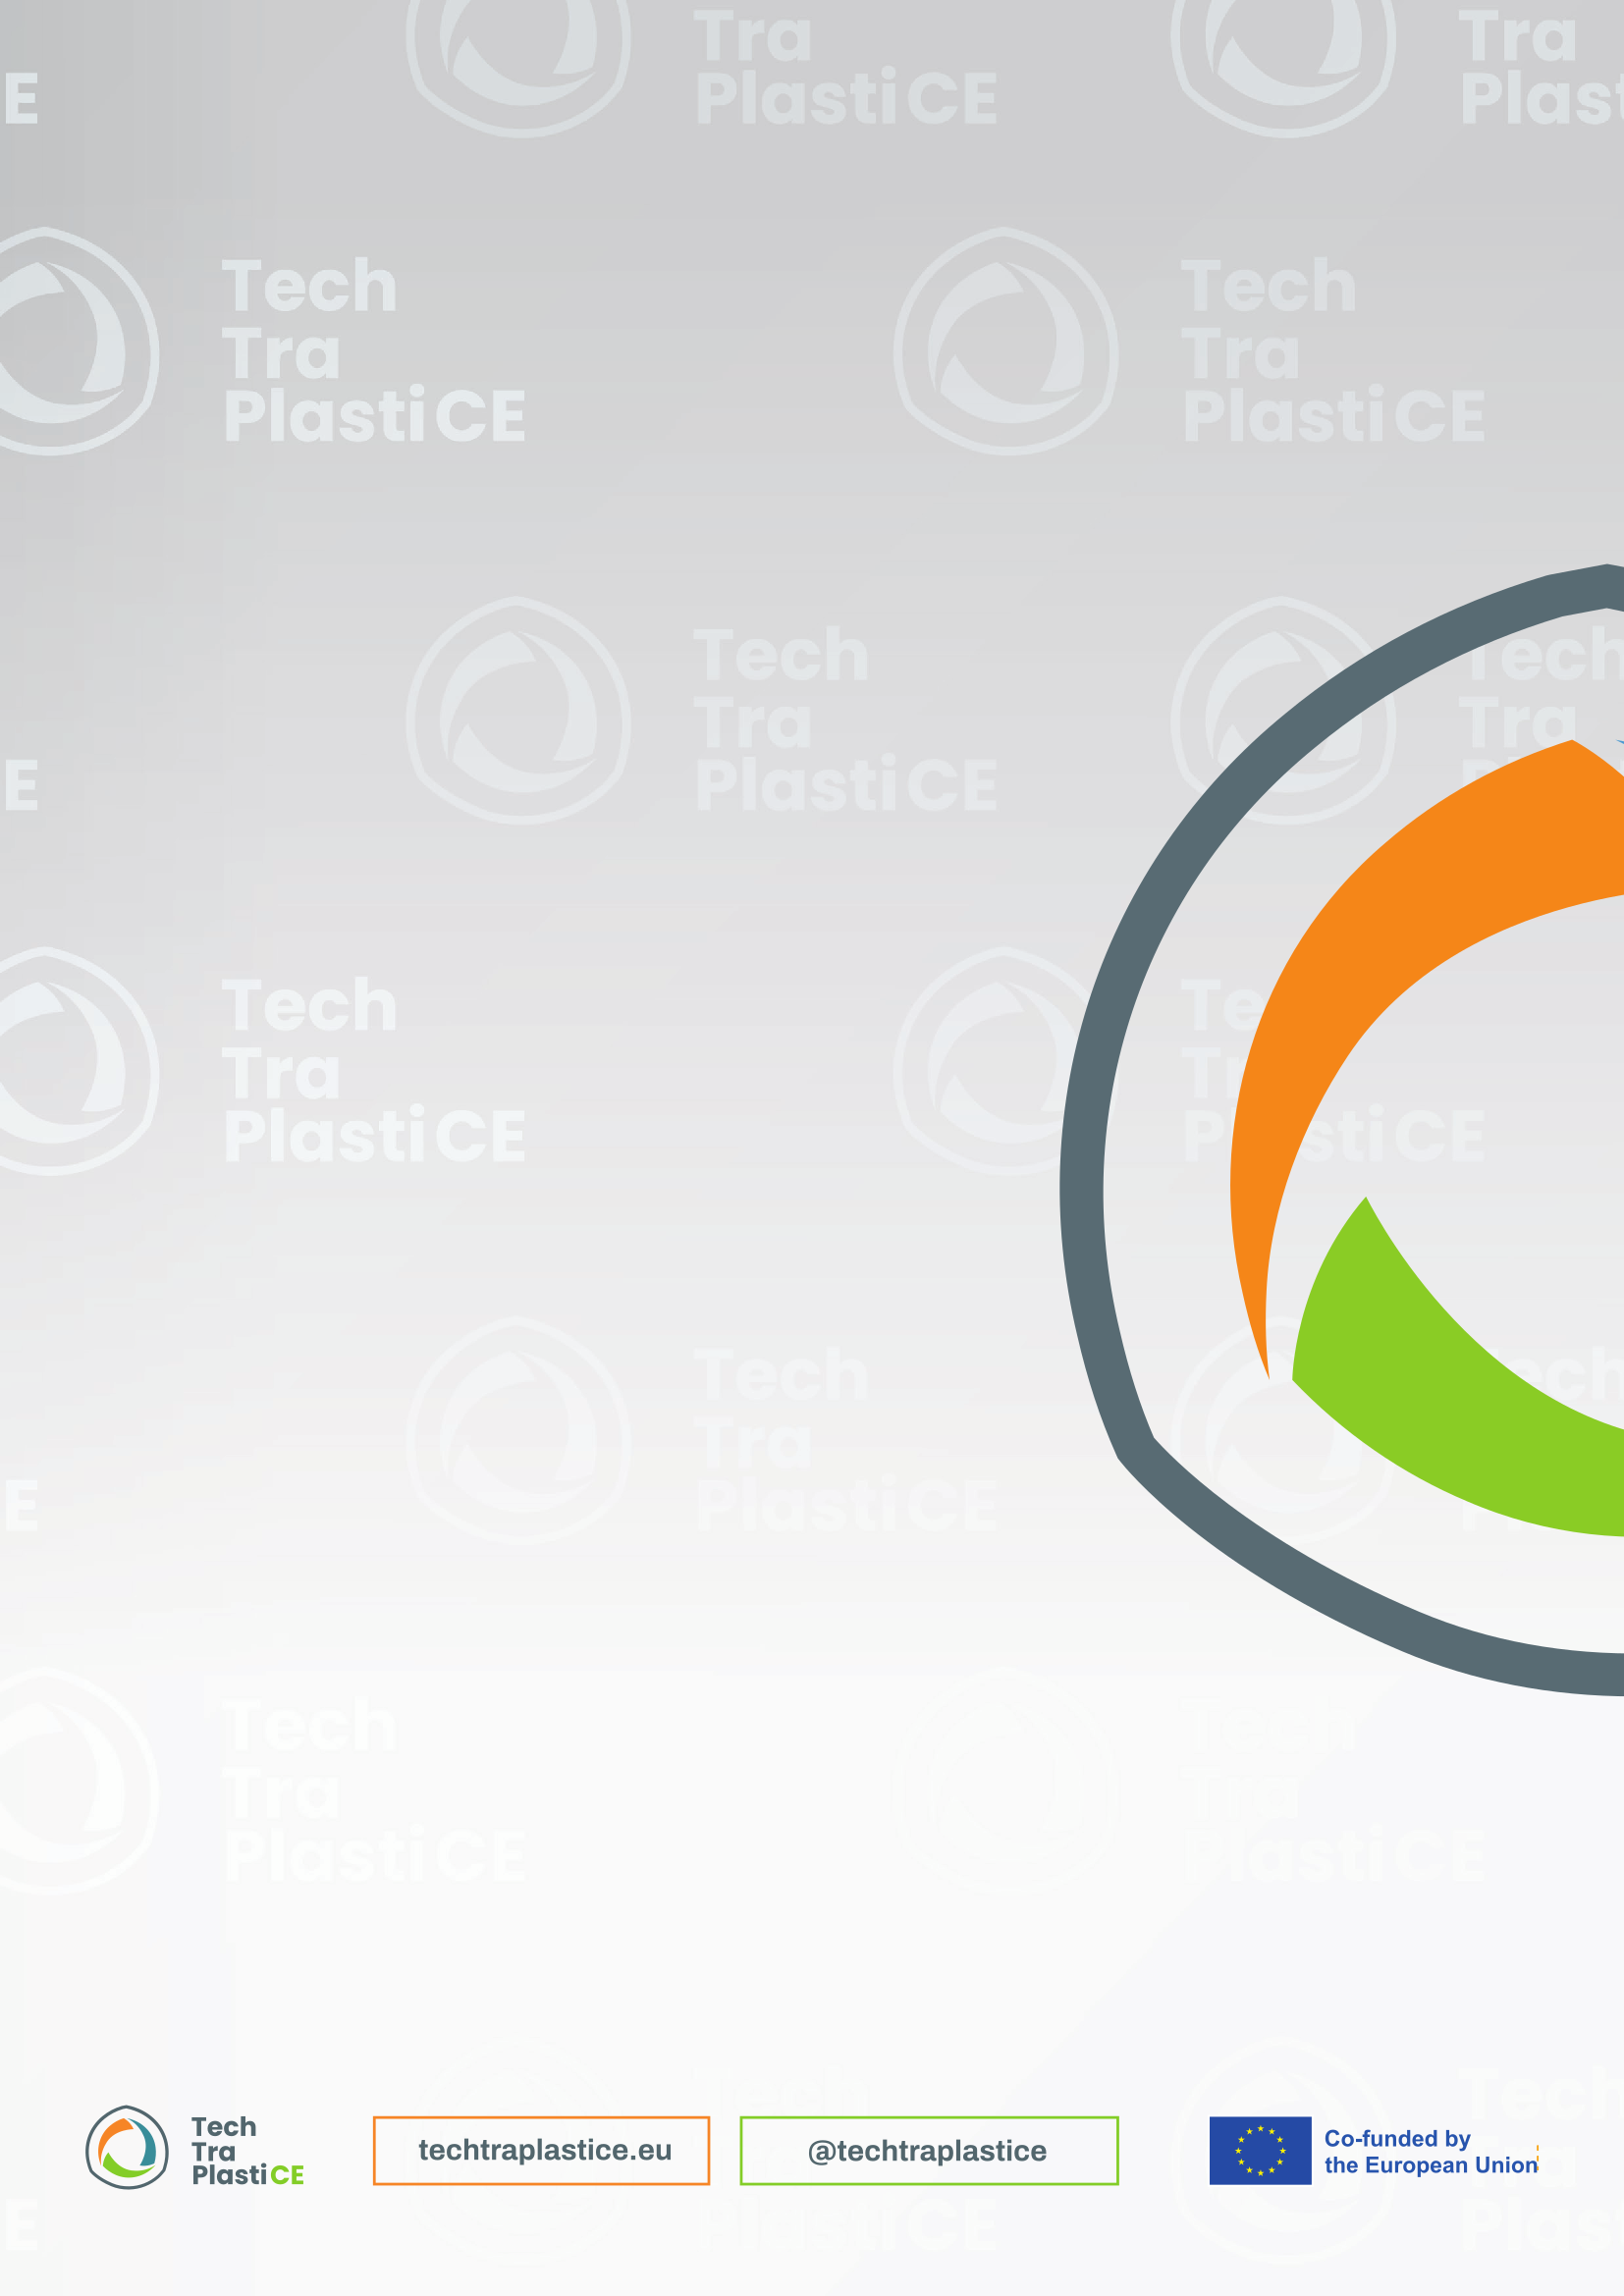
\includegraphics{assets/Portada.png}}
      }

  \BgThispage


  \begin{minipage}[b][0.78\textheight][s]{0.65\textwidth}

    \raggedright
    % Title and subtitle
    
    \vfill

    \begin{spacing}{2.2}
      {\color{Naranja}\Huge\bfseries{D2.2 Document with Portfolio
  definition by Institution}} \\[1\baselineskip] 
    \end{spacing}
    
    \begin{spacing}{1.2}
    {\color{Neutro} \Large\textit{WP2: Development of a networked
  portfolio}}\\[1\baselineskip]
    
    {\Large \color{Neutro} 
    Strengthening University Tech Transfer Capabilities to Support Circular Economy 
    Value Chains for Plastics in Latin America -
    \textsc{\centering\bfseries TechTraPlastiCE} }\\[2\baselineskip]

    
    \end{spacing}

    {\color{Neutro} \Large\textit{November 25, 2026}}
    
    \vfill
  \end{minipage}		

  \vfill

  {\scriptsize
    \color{Neutro}
    This project has been funded with the support of Erasmus +.  
    The contents are the responsibility of the author(s). 
    The Commission cannot be held responsible for any use which may be made of the information contained therein. 
    Project No. 101179564 
    }


  \newpage



  \thispagestyle{plain}
  \begin{tabu} to \linewidth {X[1.3,l]  | X[1,l] X[1,l]}
    \toprule
    \multirow{5}{*}{ 
\includegraphics[height=20mm]{assets/images/logo-TTPCE.png}} &  \textbf{Work Package} : & WP2  \\ \cmidrule{2-3}
      & \textbf{Project Number} : & 101179564  \\ \cmidrule{2-3}
      &  \textbf{Type of document}:  & Deliverable   \\ \cmidrule{2-3}
      & \textbf{Due Delivery Date}:    & April
  30/2026     \\ \cmidrule{2-3}
      & \textbf{Actual Delivery Date}:    & November 25, 2026       \\ 
    \bottomrule
  \end{tabu}

  \vfill


  \begin{tabu} to \linewidth {X[1,l]  | X[3.5,l]}
    \toprule
    \textbf{Title} : & D2.2 Document with Portfolio definition by
  Institution  \\ \cmidrule{2-2}
    \textbf{Work Package} : & WP2: Development of a networked
  portfolio  \\ \cmidrule{2-2}
    \textbf{Description} : & Each University will report the portfolio
  designed by the institutional teams following the guidelines provided
  by Universidad Nacional del Sur \& Universidade de
  Aveiro.  \\ \cmidrule{2-2}
    \textbf{Responsible} : & Universidad Nacional del Sur \&
  Universidade de Aveiro  \\ \cmidrule{2-2}
    \textbf{Author(s)} : &  
     
          Prof.~Paula Ferreira (UA), Prof.~Idalina José Gonçalves (UA),
          Prof.~Cláudia Nunes (UA).
          
          Prof.~Yamila Victoria Vazquez (UNS), Prof.~Yanela N. Alonso
          (UNS), Prof.~Luciana A. Castillo, (UNS), Econ. Yesica Soledad
          Dilernia (UNS), ID. Teresa Dutari (UNS).
           \\ \cmidrule{2-2}
    \textbf{Project Call} : & ERASMUS-EDU-2024-CBHE (Capacity building in the field of higher education)  \\ \cmidrule{2-2}
    \textbf{Dissemination Level} : & Public\\   
  \bottomrule
  \end{tabu}



  \vfill


  \begin{tabular}{ >{\raggedright\arraybackslash}p{3cm}| p{2cm} p{4cm} p{6cm} }
    \toprule
    \textbf{Version}: & \multicolumn{3}{l}{ 1.2} \\ \midrule
    \textbf{Contributors}  & Versions    & Dates       & Revision Description \\ \midrule
    UNS  & 1    & 21/04/2026  & Version 1 of the D.2.1 deliverable  \\ 
    UA  & 1.1    & 28/04/2026  & Reviewed the consolidated document and feedback on presentation of results.  \\ 
    UL  & 1.2   & 06/05/2026  & Final revision and integration of all feedback  \\ 
    \bottomrule
\end{tabular}  


    
    
    \vfill
    
    {\scriptsize\centering\color{lightgray} 
    
    Disclaimer
    
    This document is provided <<as is>> with no warranties whatsoever, 
    including any warranty or merchantability, non-infringement, fitness for any particular 
    purpose, or any warranty otherwise arising out of any proposal, specification or sample.  
    
    No license, express or implied, by estoppels or otherwise, to any intellectual 
    property rights are granted herein. 
    The members of the project TechTraPlastiCE do not accept any liability for actions or 
    omissions of TechTraPlastiCE members or third parties and disclaim any obligation 
    to enforce the use of this document. 
    
    This document reflects only the authors' view and the Commission is not responsible 
    for any use that may be made of the information it contains.  
    This document is subject to change without notice. 
    
    }
    \normalsize
    
    
    
      \end{titlepage}
  \end{frontmatter}

\renewcommand*\contentsname{Contents}
{
\setcounter{tocdepth}{2}
\tableofcontents
}
\listoffigures
\listoftables

\setstretch{1.2}
\mainmatter
\chapter*{Executive summary}\label{executive-summary}
\addcontentsline{toc}{chapter}{Executive summary}

This deliverable presents the \textbf{D2.2 Document with Portfolio
definition by Institution} of the \emph{Work Package 2 (WP2) Development
of a networked portfolio} of the TechTraPlastiCE project. The
development of institutional portfolios within the TechTraPlastiCE
project aims to transform the raw information collected in Deliverable
2.1 into structured, validated, and actionable knowledge related to the
circular economy of plastics. The report focuses on how Higher Education
Institutions (HEIs) can organize and communicate their technology
transfer capacities, services, developments, and training activities to
strengthen collaboration with industry, government, and society.

The methodology combines qualitative, comparative, and multi-level
analysis. Information gathered from partner institutions was reviewed,
standardized, and validated through the creation of ``tech cards,''
which serve as harmonized units describing services, capabilities, and
innovations associated with the plastics value chain. These cards
enabled the construction of institutional portfolios that reflect each
university's strengths, orientation, and transfer potential.

The analysis was conducted at three levels: micro (individual transfer
records), meso (institutional profiles), and macro (cross-institutional
comparison). Results reveal diverse but complementary institutional
models, ranging from highly technological and infrastructure-based
approaches to socio-territorial and sustainability-oriented profiles.
The report highlights the strategic role of universities as facilitators
of sustainable innovation and demonstrates how structured portfolios can
enhance visibility, cooperation, and impact within regional and
international circular economy ecosystems.

\chapter{Introduction}\label{introduction}

The transition towards a circular economy for plastics requires not only
the identification of innovative solutions but also the development of
structured mechanisms that enable their effective implementation within
specific institutional and territorial contexts. In this sense, higher
education institutions play a pivotal role as intermediaries between
knowledge generation and its application, particularly through their
capacity to engage with industry, public institutions, and civil
society.

The present deliverable builds upon Deliverable 2.1, which presented the
overall methodological framework of WP2 and described the tools and
processes implemented for data collection. In particular, D2.1
introduced the use of structured questionnaires, complemented by a
workshop held in Chile as well as the compilation of the raw data
collected from partner institutions. At this stage, the information was
collected but not yet subject to analytical processing. The diversity of
institutional capacities, regional contexts, and stakeholder ecosystems
across the consortium requires a more tailored and strategic approach to
ensure that these offers are not only relevant but also implementable
and sustainable.

Within this context, \emph{the objective of D2.2 is to show the
transformation process from this collected information into structured
and comparable knowledge. This involves the characterization of
institutional profiles, the identification of patterns in technology
transfer activities, and the construction of institutional service
portfolios related to the core of the project, ``plastic value chain at
the circular economy''}. The methodological approach of this deliverable
combines qualitative and comparative analysis, enabling the
transformation of the information collected in D2.1 into structured and
actionable knowledge. The approach is organized across three
complementary levels of analysis: (i) a micro level, focused on the
detailed examination of individual technology transfer records; (ii) a
meso level, oriented toward the aggregation and characterization of
institutional profiles; and (iii) a macro level, based on comparative
analysis across universities, countries, and the consortium as a whole.

A key element of this process was the constitution of \textbf{technology
cards} (tech cards from now on), which function as standardized units to
organize and systematize the identified capacities, enabling their
subsequent aggregation into institutional portfolios. Each
\emph{service, capability, training activity, or development} identified
in the repository (D2.1) was translated into a tech card, ensuring a
consistent description in terms of its characteristics, scope, type of
activity, and potential application within the plastics value chain.
This validation and standardization process not only improved the
clarity and comparability of the information, but also created a common
analytical basis across all partner institutions. A central aspect of
this process is the recognition that effective technology transfer
requires moving beyond fragmented and \emph{ad hoc} interactions towards
more structured, visible, and demand-driven service offerings.

As a result, the tech cards function as the building blocks for the
subsequent construction of institutional portfolios, enabling a
structured transition from a general inventory of capacities to targeted
and actionable service offerings. In this sense, universities can
improve their capacity to communicate their expertise, engage with
external stakeholders, and respond strategically to emerging challenges
in the plastic value chain.

\begin{figure}[H]

\centering{

\pandocbounded{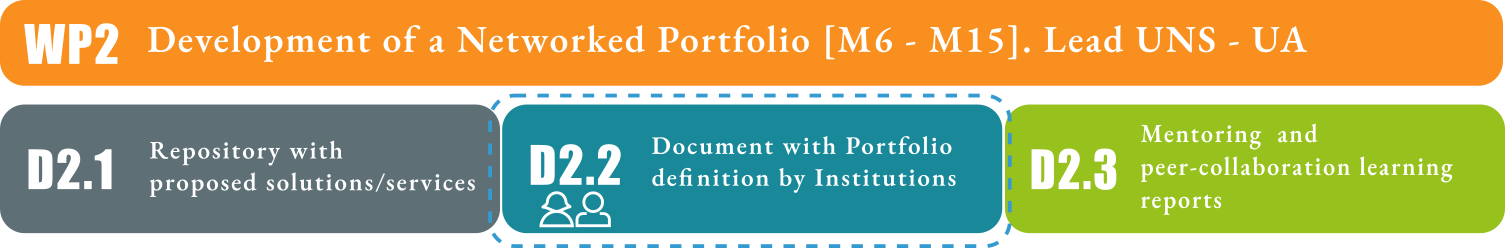
\includegraphics[keepaspectratio,alt={alt}]{figures/2.2/D2.2.png}}

}

\caption{\label{fig-baseline}Deliverable \emph{D2.2 Portfolio definition
for each HEIs}}

\end{figure}%

\chapter{Methodological Approach}\label{methodological-approach}

The present deliverable is based on a comprehensive methodological
approach that combines qualitative and comparative analysis to examine
and structure technology transfer capacities identified within the
framework of the circular economy of plastics. The overall objective is
to transform the information collected in D2.1 into structured and
actionable knowledge, enabling: (i) the characterization of
institutional profiles, (ii) the identification of patterns and trends
in technology transfer activities, and (iii) the development of coherent
and operational service portfolios at the institutional level. The
analytical process was structured across three complementary levels:

\begin{itemize}
\tightlist
\item
  \textbf{Micro level}: focused on the individual analysis of each tech
  card, allowing a detailed examination of specific capacities and
  services.
\item
  \textbf{Meso level}: oriented towards the aggregation and analysis at
  the institutional level, enabling the characterization of each
  university's portfolio and transfer profile.
\item
  \textbf{Macro level}: based on comparative analysis across
  universities, countries, and the consortium as a whole, facilitating
  the identification of broader patterns, complementarities, and
  strategic opportunities.
\end{itemize}

This methodological approach responds to the need to move from a
descriptive repository of services towards a more analytical and
strategic understanding of how universities operate as technology
transfer actors within their respective ecosystems. Through this
multi-level analytical framework, the deliverable not only structures
institution-specific portfolios but also identifies patterns, trends,
and complementarities in technology transfer activities. Indeed, this
deliverable acknowledges the heterogeneity of the participating
institutions and the importance of contextualization. In this sense, the
methodology not only organizes information but also provides a framework
for interpretation, comparison, and decision-making.

Each university operates within a distinct regulatory, economic, and
industrial landscape, which influences both the nature of the challenges
faced and the opportunities for intervention. Therefore, the portfolio
definition process is inherently context-sensitive, allowing each
institution to prioritize and adapt services according to its specific
strengths, strategic objectives, and local stakeholder needs.
Ultimately, D2.2 represents a key step in bridging the gap between
knowledge and action within the TechTraPlastiCE project. This
multi-level approach ensures both depth and comparability, allowing the
analysis to capture the complexity and diversity of technology transfer
practices across the consortium by organizing a wide range of potential
solutions into structured service portfolios within institutional
frameworks.

The work carried out through WP2 reinforces the role of higher education
institutions as key actors in advancing a circular economy for plastics
at micro, meso and macro level (as illustrated in
Figure~\ref{fig-method} ), increasing their capacity to deliver tangible
impacts at regional and international scales.

\begin{figure}[H]

\centering{

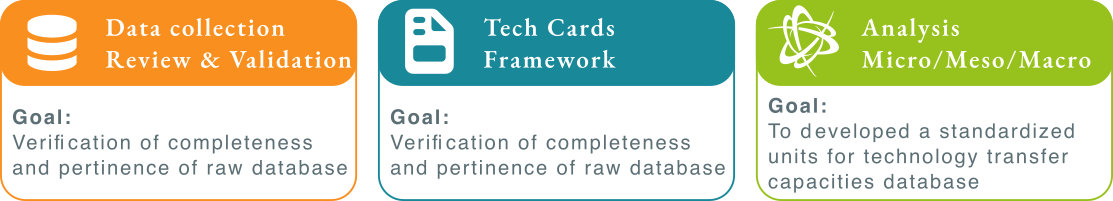
\includegraphics[width=0.9\linewidth,height=\textheight,keepaspectratio]{figures/2.2/Method-2.2.png}

}

\caption{\label{fig-method}Methodological approach for portfolio
definition for HEIs}

\end{figure}%

\section{Data collection, review, and
validation}\label{data-collection-review-and-validation}

The first stage of the methodological process consisted of a systematic
review of the data provided by the partner institutions, included in
D2.1 in the annexes. All forms submitted by the member universities were
individually analyzed, corresponding to technology transfer capacities
related to the circular economy of plastics across the four key axes:
\emph{services, capabilities, training, and developments}. This stage
aimed to ensure the quality, reliability, and comparability of the
dataset. To achieve this, several tasks were carried out:

\begin{itemize}
\tightlist
\item
  Verification of data completeness and internal consistency,
\item
  Review of the categorization assigned to each entry,
\item
  Identification of inconsistencies and suggestion of reclassification
  where necessary (e.g., distinguishing between services and
  capabilities),
\item
  Revision and harmonization of language to ensure clarity, coherence,
  and accessibility for different types of stakeholders, including
  non-technical audiences.
\end{itemize}

This process was essential to reduce ambiguity and heterogeneity in the
data, which are common challenges in multi-institutional projects.
Subsequently, a second validation stage was conducted, involving direct
feedback from each partner institution. Universities were invited to
review, adjust, and confirm the information corresponding to their
original submissions with modifications and suggestions made by WP2
members. This iterative validation process ensured both internal
consistency and alignment with project criteria, while also
strengthening institutional ownership of the results.

\section{Construction of tech cards and institutional
portfolios}\label{construction-of-tech-cards-and-institutional-portfolios}

Based on the validated dataset, tech cards were developed as
\emph{standardized units for recording and structuring technology
transfer capacities}. These cards constitute the core analytical tool of
this deliverable, enabling the transformation of heterogeneous
information into a consistent and comparable format. Each tech card
captures key attributes of a given capacity, including its type, scope,
orientation, and potential application. This standardization facilitates
both the analysis and communication of institutional capabilities.

A total of \textbf{303 tech cards} were compiled, representing a broad
spectrum of activities across the consortium. These tech cards were
written in both English and Spanish. From this dataset, institutional
portfolios were constructed by organizing the cards according to the
type of activity (services, developments, training, and capabilities).
These portfolios are not conceived as simple inventories, but as
structured representations of each institution's potential contribution
to the plastic value chain. They reflect both the diversity and
specialization of capacities, providing a foundation for strategic
engagement with external stakeholders.

\section{Institutional-level analysis (micro \& meso
level)}\label{institutional-level-analysis-micro-meso-level}

A systematic and comparative analysis of tech cards (micro level) was
performed in order to obtain a detailed examination of specific
capacities and services. This analysis also allowed the organization of
tech cards according to a set of analytical criteria. This
categorization process was essential to transform qualitative
information into analyzable variables.

The main criteria included:

\begin{itemize}
\tightlist
\item
  \textbf{Type of activity}: services, developments, training, and
  capabilities,
\item
  \textbf{Orientation of the transfer}: technical/technological, social,
  innovation-oriented, training/educational, or hybrid,
\item
  \textbf{Nature of the capacity}: knowledge-based,
  infrastructure-based, technical assistance, among others.
\end{itemize}

This multi-dimensional classification allowed the construction of
analytical variables that facilitated cross-institutional comparison and
pattern identification. Moreover, it enabled the identification of
dominant orientations and the balance between different types of
activities within each institution.

At the meso level, the analysis focused on the characterization of each
university's profile based on its portfolio of technology transfer
capacities. This involved examining the distribution of tech cards by
type of activity, the predominant orientation of transfer activities,
and the balance between services, developments, capabilities, and
training components. This analysis facilitated the identification of
institutional trends and strategic orientations. For instance, some
universities exhibited a strong focus on service provision and technical
assistance, while others demonstrated a strong experience in
technological developments or training activities. Based on these
patterns, a typology of universities was developed, classifying them
according to their dominant transfer profile, such as
technical/technological-oriented, social-oriented, innovation-driven,
training/educational-oriented, or hybrid. This typology provides a
useful framework for understanding institutional roles within the
consortium and for identifying potential complementarities.

\section{Comparative analysis and pattern identification (macro level),
and consortium profile
analysis}\label{comparative-analysis-and-pattern-identification-macro-level-and-consortium-profile-analysis}

At the macro level, a comparative analysis across universities was
conducted to identify patterns and trends at both, country and regional
levels. This stage aimed to go beyond individual institutional analysis
and capture systemic dynamics within the consortium. The analysis
included the comparison of institutional profiles, identification of
similarities and differences between portfolios, and detection of areas
of specialization and potential complementarities. To facilitate this
process, institutions were grouped by country, considering each national
context as a cluster. This approach allowed the identification of
territorial trends, including common strengths, shared challenges, and
potential influences of regulatory, economic, or institutional
environments. Such comparative insights are particularly relevant for
designing context-sensitive strategies and fostering cross-country
collaboration.

Finally, an integrated analysis of all portfolios was conducted to
characterize the overall profile of the consortium. This holistic
perspective allowed us to identify collective strengths and consolidated
areas of expertise across institutions, detect gaps or underrepresented
domains that may require further development or strategic reinforcement,
and recognize complementarities among institutions, highlighting
opportunities for collaboration and synergies within the network. In
addition, this comprehensive analysis enabled a better understanding of
how different types of transfer capacities, such as services,
technological developments, training activities, and capabilities, are
distributed and interconnected across the consortium, providing insights
into the overall balance and orientation of technology transfer
activities.

\chapter{Results and discussion}\label{results-and-discussion}

\section{Form validation}\label{form-validation}

A total of 303 forms were received (per language, Spanish and English)
from the partner universities, distributed across four main axes:
services, capabilities, developments, and training. These forms
represent the initial dataset describing the technology transfer
capacities of the partner institutions within the framework of the
circular economy of plastics.

Following a detailed review and analysis of the submitted forms, a
subset of entries was reassigned to a different category. This
reclassification process was necessary to ensure consistency in the
categorization criteria, as some submissions presented overlaps or
ambiguities between categories. The reassignment was carried out based
on a standardized set of definitions and classification guidelines
established within the work package, aiming to improve the comparability
and analytical robustness of the dataset. This validation stage played a
key role in enhancing the overall quality and reliability of the
information, allowing for a more accurate representation of
institutional capacities. It also contributed to harmonizing the
interpretation of categories across partner institutions, which is
particularly relevant in a multi-country and multi-institutional
context.

Figures 1-4 present the distribution of forms across the four dimensions
for each university, separated by regions, within the consortium.
Additionally, when applicable, it indicates the number of forms that
were reassigned from their original category, providing transparency
regarding the adjustments made during the validation process. This
structured and validated dataset constitutes the basis for the
subsequent construction of technology cards and the development of
institutional portfolios, ensuring that the analysis is grounded on
consistent, comparable, and high-quality information.

Based on the verification of the information provided, a brief analysis
is presented below, highlighting the main suggestions and modifications
made to the original data prior to its validation by each institution.
This analysis focuses on identifying the most relevant adjustments
carried out during the data review process, including improvements in
categorization, clarification of descriptions, and alignment with the
established criteria of the project. The purpose of these modifications
was to enhance the consistency, clarity, and comparability of the
information across all partner institutions. The revised data was
subsequently shared with each university for validation, allowing them
to review, confirm, and, where necessary, refine the proposed changes.
This iterative process ensured that the final dataset accurately
reflects the institutional capacities while maintaining coherence with
the overall methodological framework of the deliverable.

From the comparison between the initial and final distribution of forms
across the four dimensions (Figure~\ref{fig-CO} - Figure~\ref{fig-EU} ),
different patterns of adjustment among regions and institutions can be
observed, reflecting varying levels of consistency in the original data
classification. In the case of the Colombian universities
(Figure~\ref{fig-CO}), UC and UNAL, no differences were observed between
the initial and final distributions in any of the dimensions. All
categories remained unchanged, indicating that no reassignment, removal,
or adjustment was required during the validation process. This stability
suggests a high level of coherence in the original classification of the
forms and an adequate understanding of the methodological criteria from
the outset.

\begin{figure}[H]

\centering{

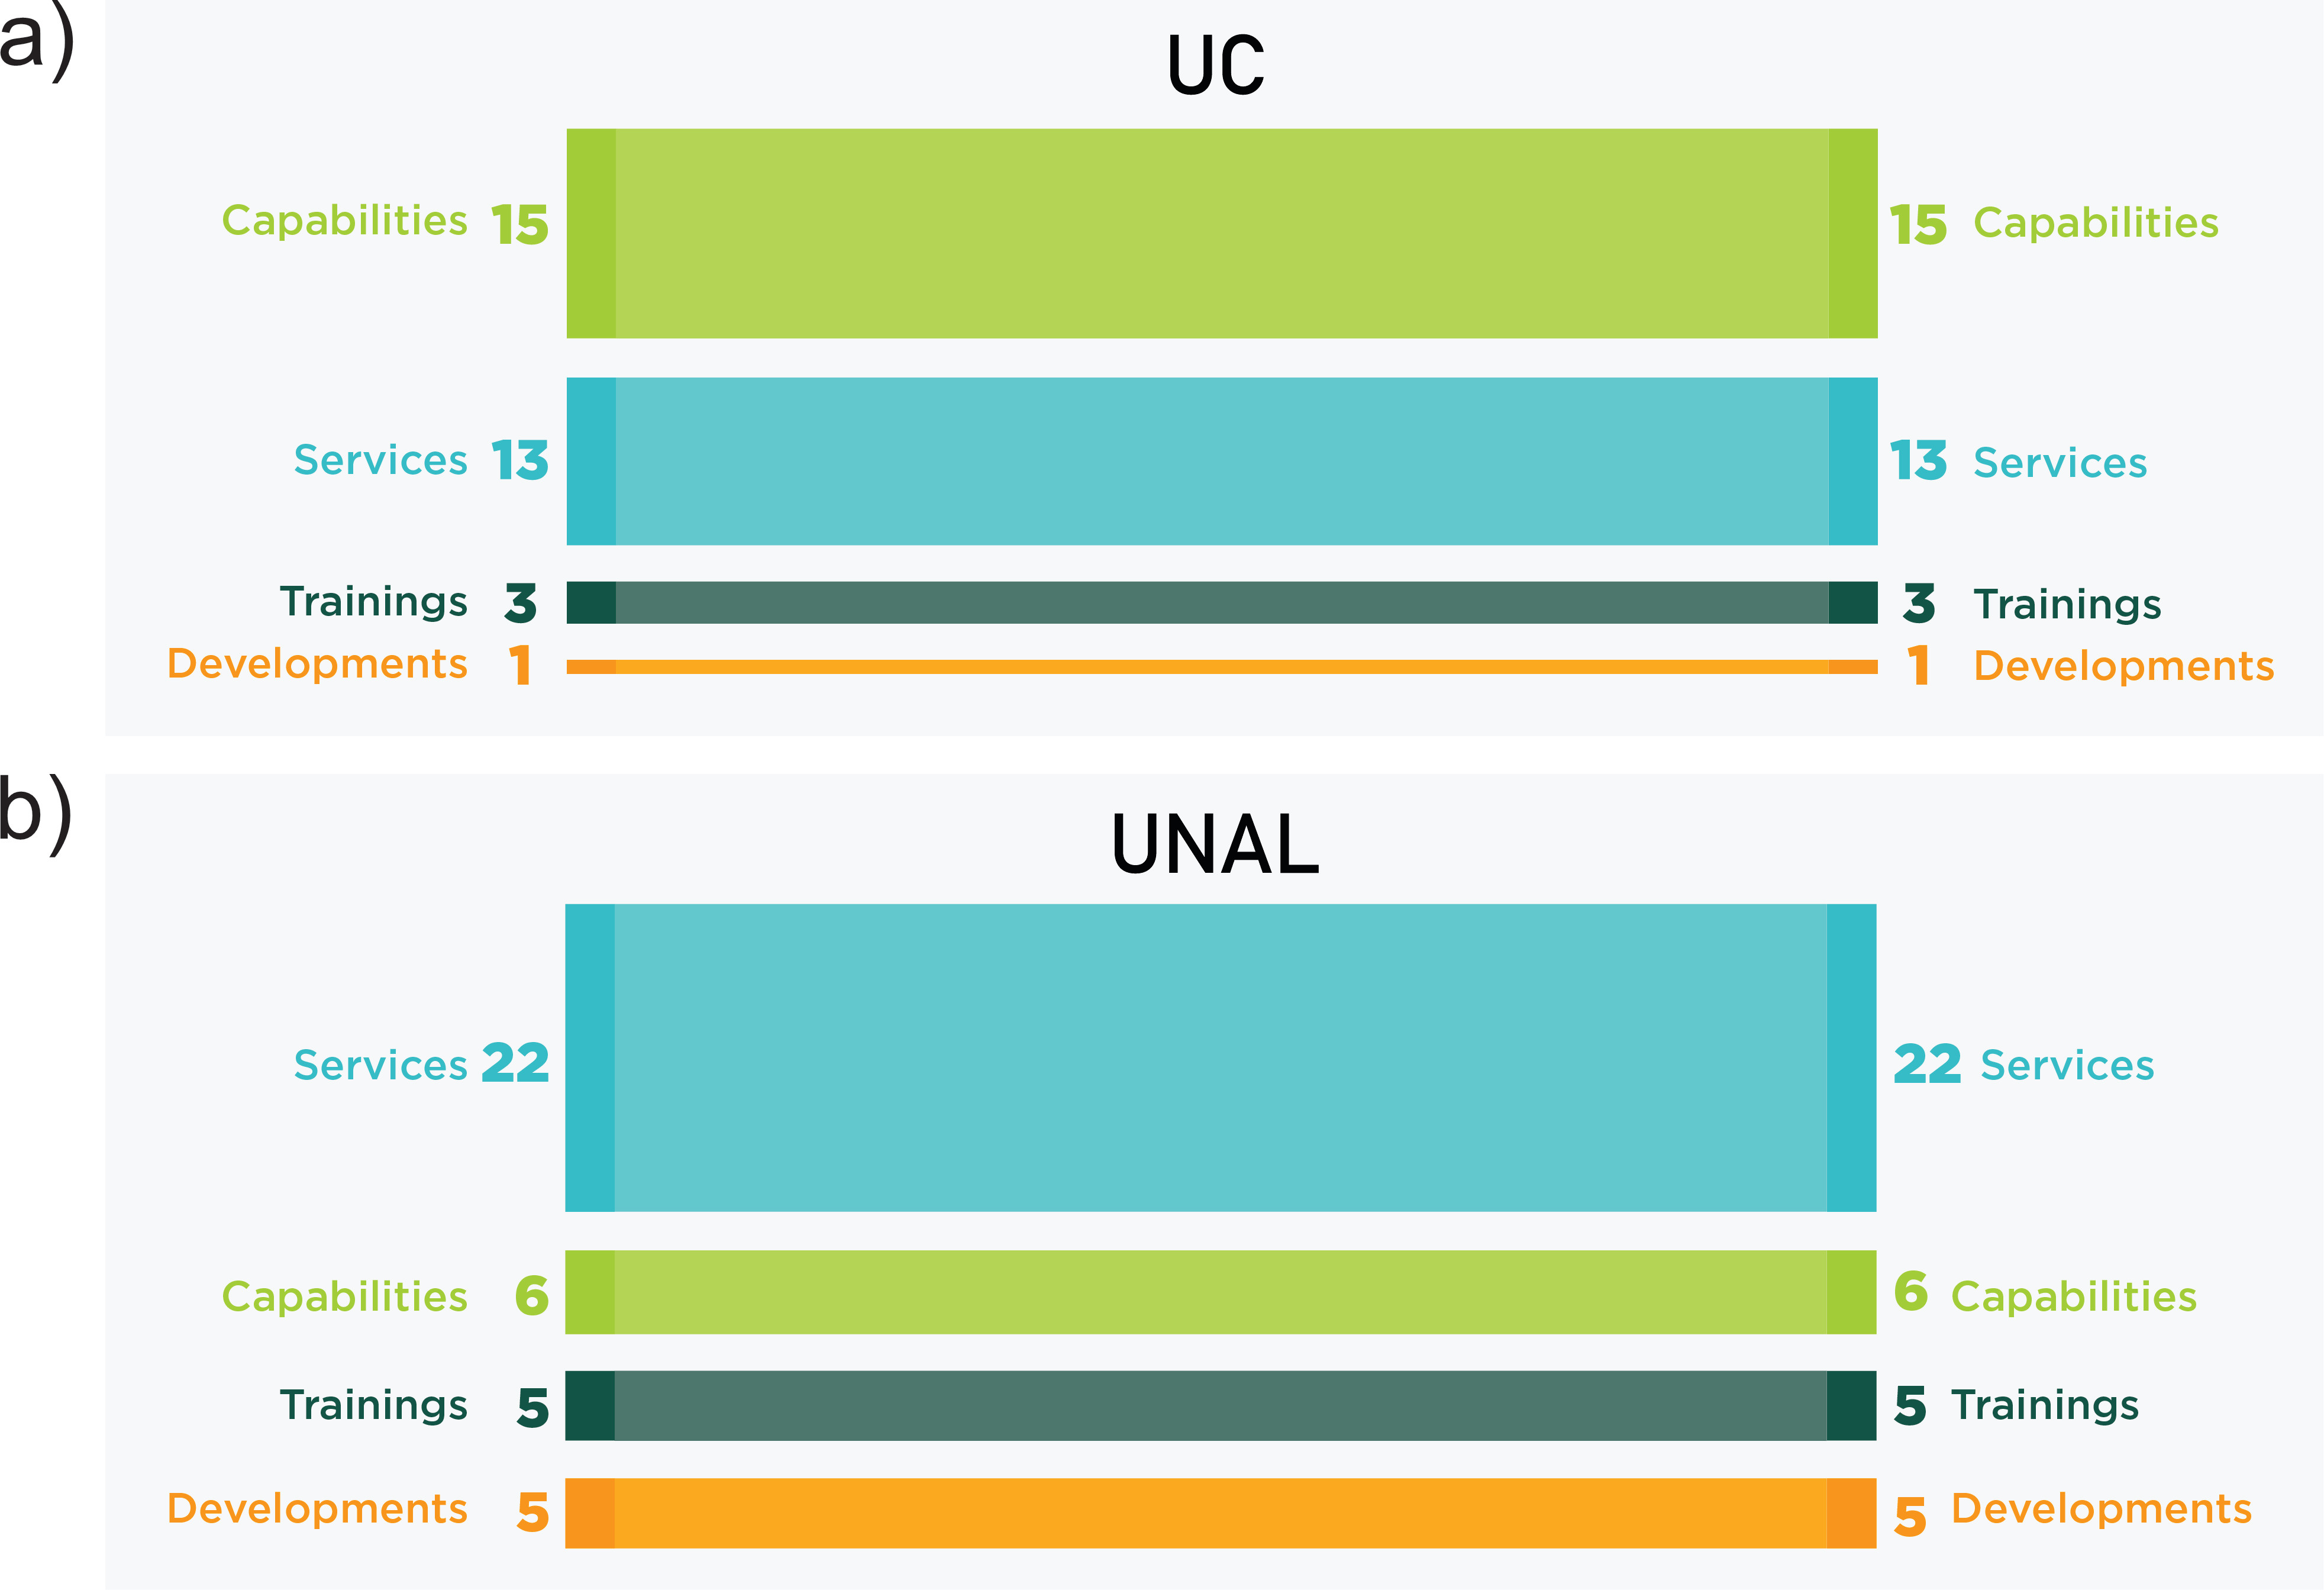
\includegraphics[width=0.8\linewidth,height=\textheight,keepaspectratio]{figures/2.2/1.jpg}

}

\caption{\label{fig-CO}Number of received forms, of the different axes,
from the Colombian universities ((a) UC and (b) UNAL) and final
distribution after processing the content.}

\end{figure}%

A different situation is observed in the Chilean universities
(Figure~\ref{fig-CH}), where the most significant adjustments took
place. In the case of PUCV, a clear reassignment process was identified,
with four forms being reclassified from Services to Capabilities
(Services: 10 to 6; Capabilities: 4 to 8), while Developments and
Trainings remained unchanged. This indicates an initial ambiguity in the
distinction between service provision and institutional capacities,
which was resolved during the validation process. For USACH, the
adjustments involved both data cleaning and reassignment. Services
decreased from 25 to 24 due to the removal of a duplicated form, while
Trainings increased from 3 to 5 since 2 services were also potential
training courses. Capabilities and developments remained stable at 14,
indicating consistency in this dimension.

\begin{figure}[H]

\centering{

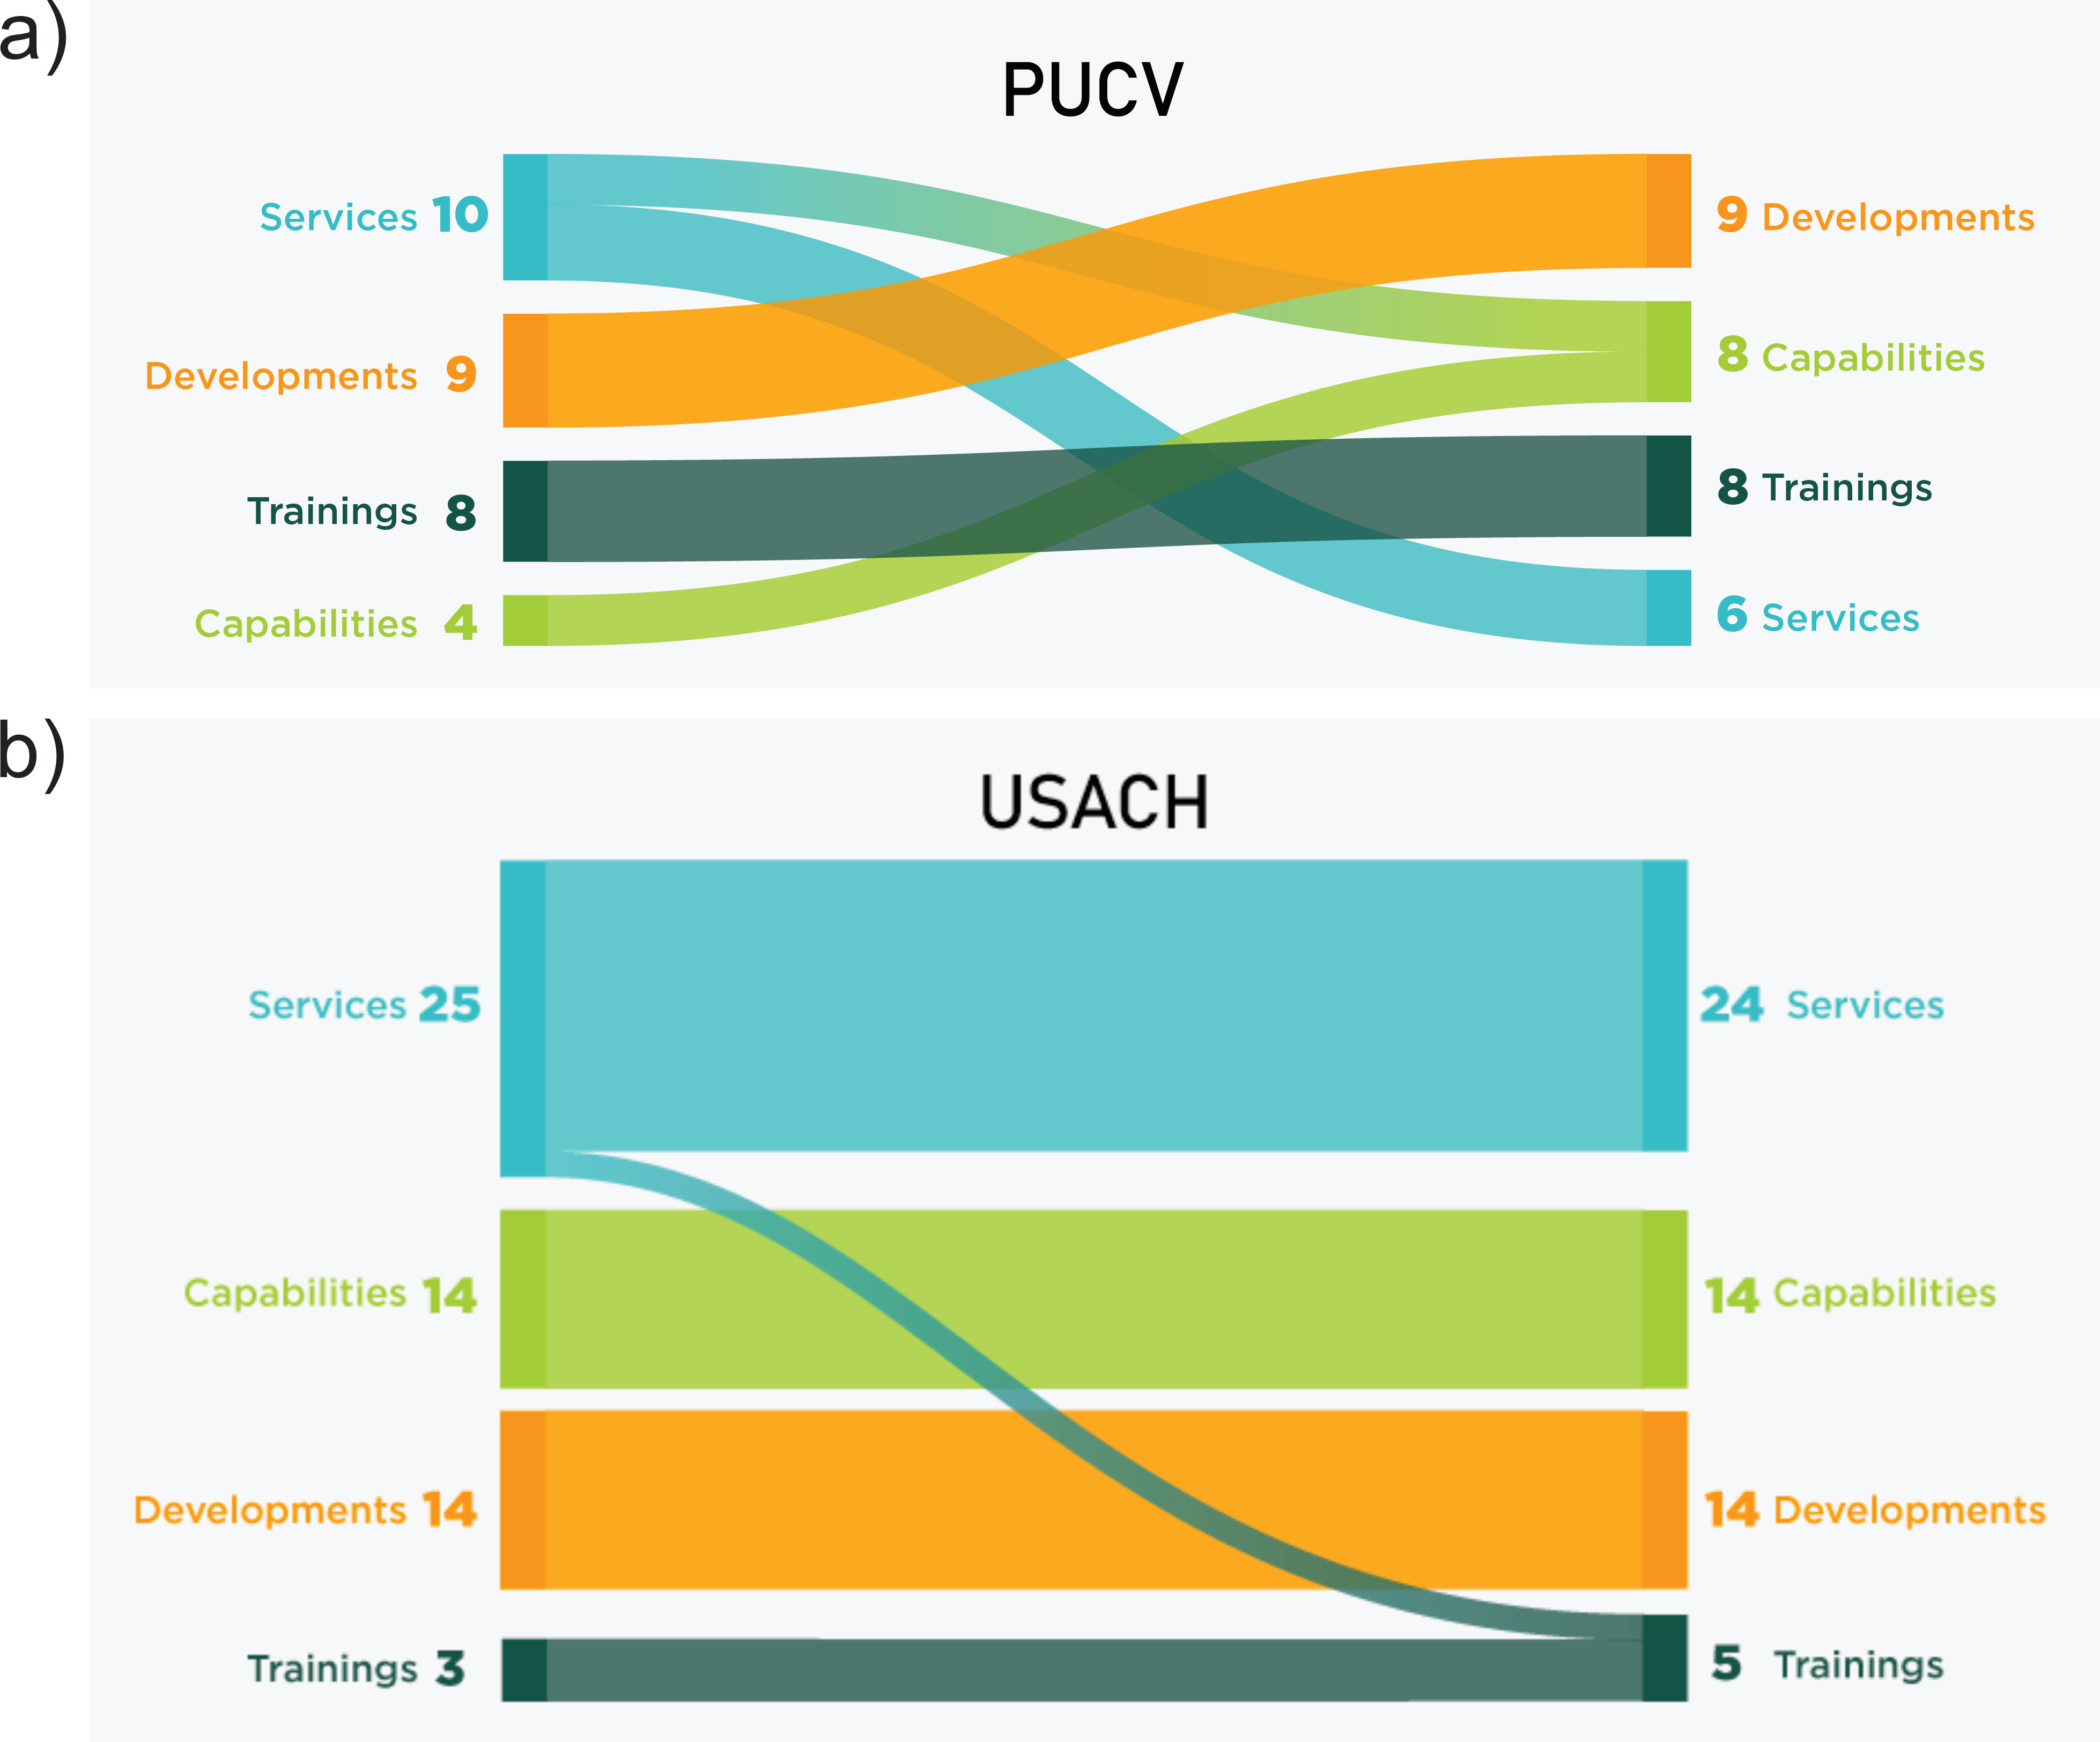
\includegraphics[width=0.8\linewidth,height=\textheight,keepaspectratio]{figures/2.2/2.jpg}

}

\caption{\label{fig-CH}Number of received forms, of the different axes,
from the Chilean universities ((a) PUCV and (b) USACH) and final
distribution after processing the content.}

\end{figure}%

Regarding the Argentinian universities (Figure 3), most institutions
showed a high level of stability. Both UNC and UNS presented no changes
between the initial and final distributions, confirming the consistency
of their original classifications. In contrast, UNRN exhibited a minor
adjustment, with one form being reassigned from Capabilities to
Developments (Capabilities: 5 to 4; Developments: 2 to 3), while the
remaining dimensions remained unchanged. This represents a targeted
refinement rather than a structural inconsistency.

\begin{figure}[H]

\centering{

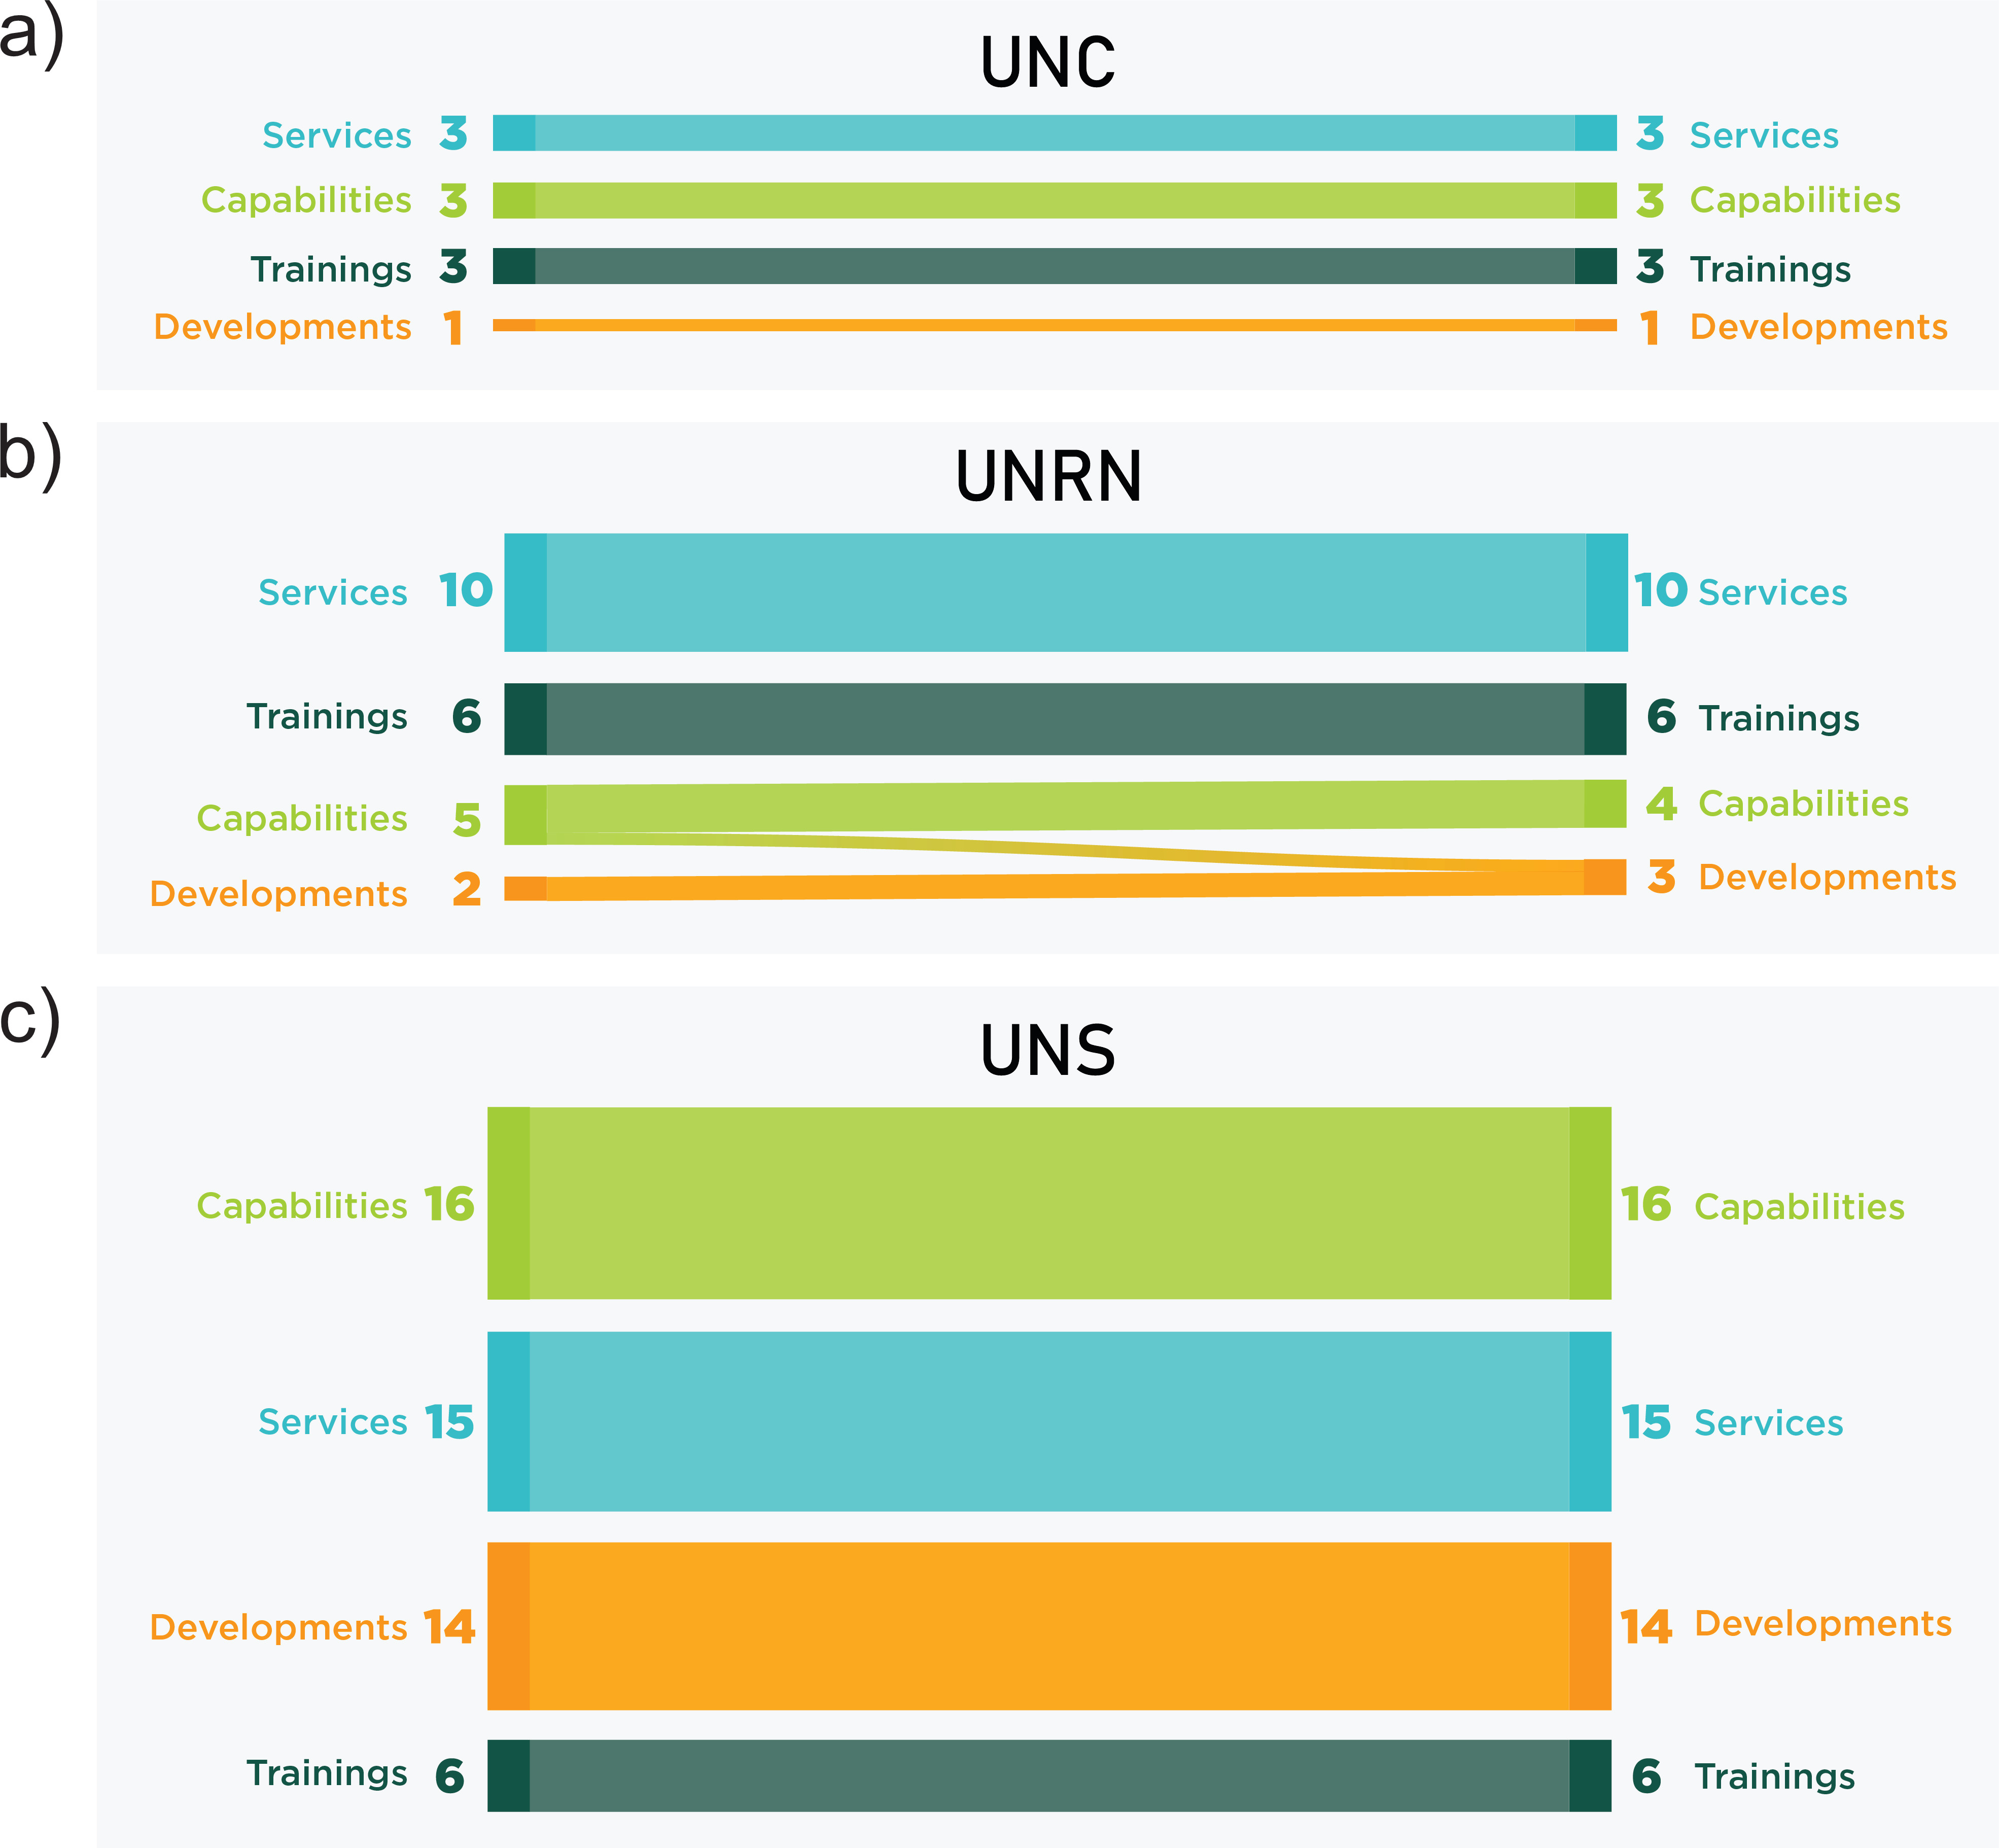
\includegraphics[width=0.8\linewidth,height=\textheight,keepaspectratio]{figures/2.2/3.jpg}

}

\caption{\label{fig-AR}Number of received forms, of the different axes,
from the Argentinian universities ((a) UNC, (b) UNRN, and (c) UNS) and
final distribution after processing the content.}

\end{figure}%

Finally, in the case of the European universities (Figure~\ref{fig-EU}),
UL and UA, no reassignment processes were identified, and the
distributions remained unchanged after validation. This indicates that
the initial categorization was fully aligned with the methodological
framework.

Furthermore, opportunities for improvement were identified in the
descriptive quality of the forms. In several cases, it was necessary to
clarify the information provided to ensure a consistent interpretation
across institutions. This included the reformulation of descriptions,
the incorporation of missing technical details, and the removal of
redundancies, contributing to greater clarity and comparability of the
data. Another significant adjustment was related to aligning the content
with the methodological criteria of the project. This involved reviewing
the relevance of each form within the established conceptual framework,
ensuring that all records met the standards defined for the development
of technology cards and institutional portfolios.

This validation process, combining reassignment, clarification, and data
cleaning where necessary, ensured the consolidation of a robust,
coherent, and comparable dataset across all partner institutions,
providing a reliable basis for the subsequent development of technology
cards and institutional portfolios.

\begin{figure}[H]

\centering{

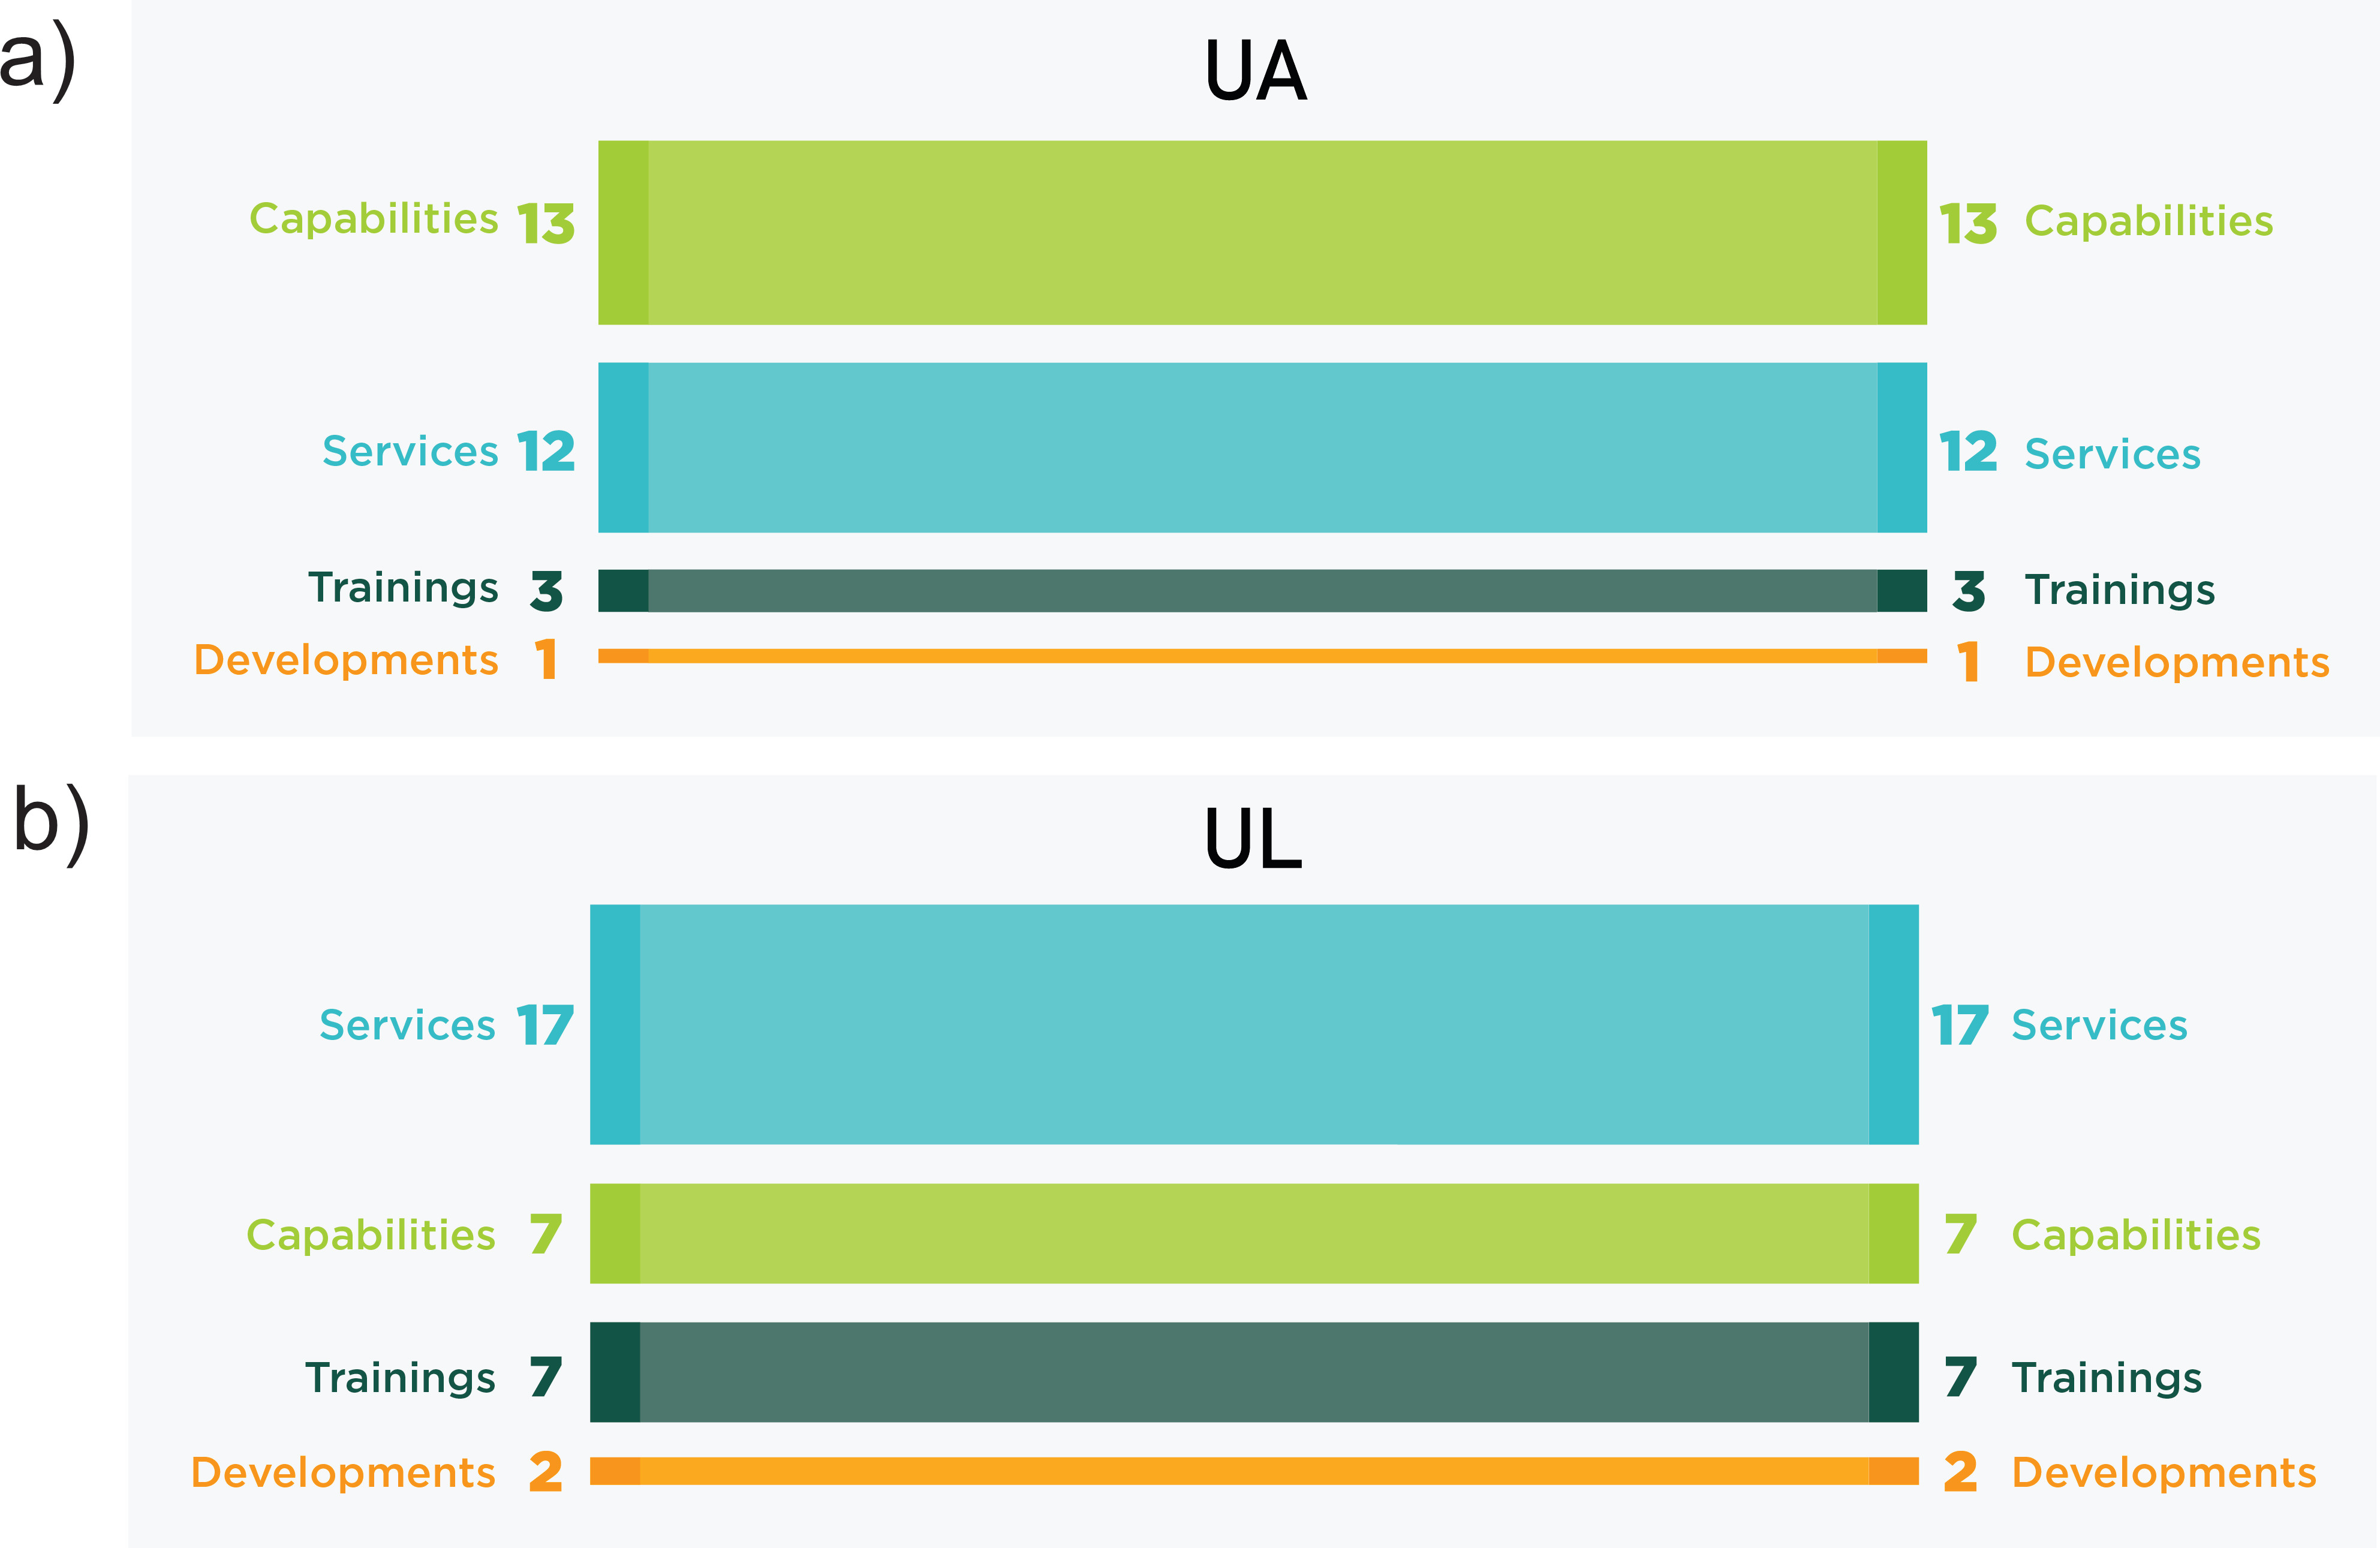
\includegraphics[width=0.8\linewidth,height=\textheight,keepaspectratio]{figures/2.2/4.jpg}

}

\caption{\label{fig-EU}Number of received forms, of the different axes,
from the European universities ((a) UA and (b) UL) and final
distribution after processing the content.}

\end{figure}%

\section{Tech Cards}\label{tech-cards}

Figure~\ref{fig-tech} presents the structure of the tech cards that
constitute the analytical foundation of this deliverable and enable the
structuring of each institution's technology transfer offer in
comparable terms. For this reason, the way in which information is
presented within each card is key to facilitating its readability and
interpretation. The Figure~\ref{fig-tech} illustrates the templates used
for the development of the tech cards considering the visual identity of
TechTraPlastiCE

\begin{figure}[H]

\centering{

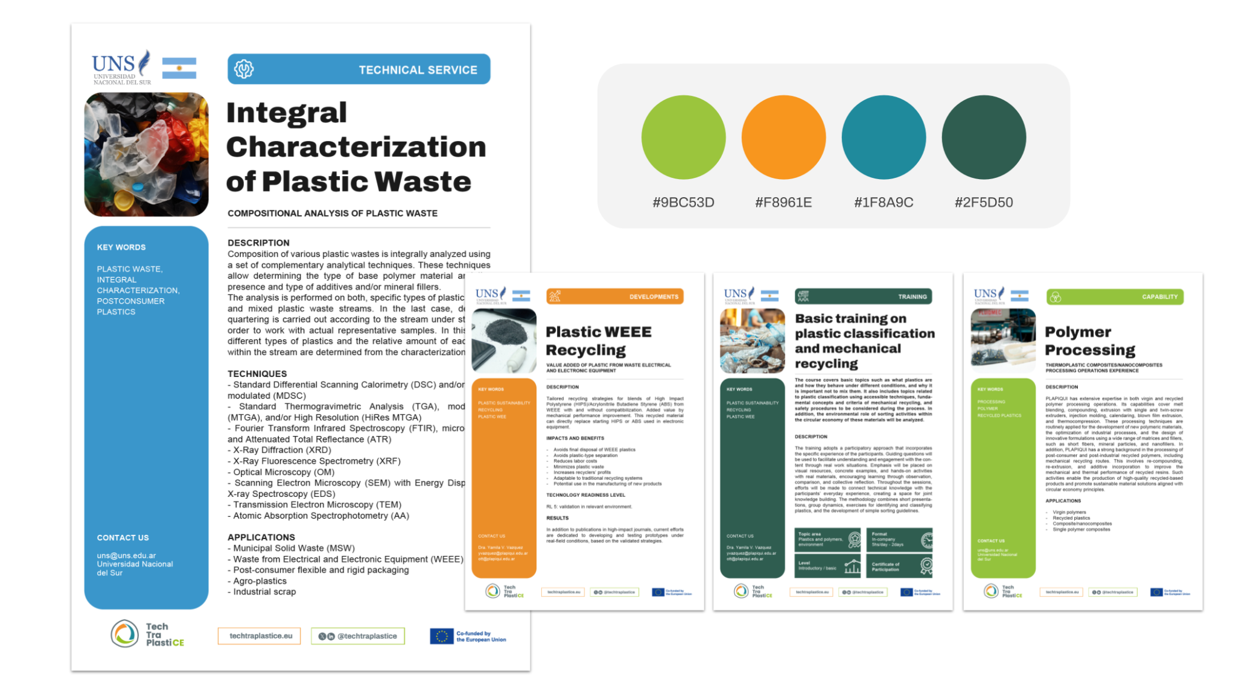
\includegraphics[width=1\linewidth,height=\textheight,keepaspectratio]{figures/2.2/5.png}

}

\caption{\label{fig-tech}Templates used for the tech cards for services,
capabilities, developments, and training.}

\end{figure}%

As can be observed in Figure~\ref{fig-tech}, the design of the tech
cards is consistent across all cases, incorporating a color-coded
identification system according to each thematic axis. This approach
ensures visual coherence throughout the set while facilitating the rapid
identification of information by the user. Based on the information
collected from the forms, a format was developed to synthesize and
organize the content clearly within a single page. Initially, the
possibility of developing an individual web page for each card was
considered. However, given the number of cases and the available
timeframe, a downloadable \texttt{PDF} format was selected. This format
ensures accessibility, portability, and ease of dissemination through
different communication channels.

The design is structured around four colors, one for each axis
(Capabilities, Developments, Services, and Training), defined in
alignment with the project's visual identity. Each technology card
features a header with the corresponding color, accompanied by the name
of the axis and a representative icon. In terms of visual hierarchy, the
title is prioritized as the main element, followed by a subtitle that
expands on the information. A representative image is also included to
complement the content, along with a brief description summarizing the
development, service, training activity, or capacity presented. On the
side section, highlighted with a color-coded background, keywords and
contact information are displayed, allowing quick access to relevant
details. At the bottom of the card, the project's institutional logos
are included, along with references to the website and social media
channels, ensuring traceability and connection with the broader project
ecosystem.

During the design process, several exchange and feedback sessions were
conducted with the team from UNRN, leaders of WP5, which enabled the
incorporation of improvements and validation of the proposed format. As
a result of these interactions, additional elements were integrated,
such as the institutional identification (logo) of each participating
university and the inclusion of the corresponding national flag, both
positioned at the top of the card. Furthermore, the inclusion of
clickable links within the PDF format was considered, allowing direct
access to institutional and project websites, thus enhancing usability
and interactivity. Regarding visual identity, the color palette was
refined to align with the project's guidelines, defining the following
colors for each axis: Capabilities (\#9BC53D
\textcolor{Verde}{\scalebox{1}{$\blacksquare$}}), Developments (\#F8961E
\textcolor{Naranja}{$\blacksquare$}), Services (\#1F8A9C
\textcolor{Celeste}{$\blacksquare$}), and Training (\#2F5D50
\textcolor{Verde_osc}{$\blacksquare$}).

Finally, the system for developing the tech cards was based on an
editable PowerPoint template. In an initial stage, this template was
designed to establish a common structure, defining criteria for visual
hierarchy, information organization, and graphic guidelines. In a second
stage, different members of WP2 used this template to complete the
content of each tech card based on the information collected from the
forms. This workflow allowed the distribution of tasks among teams while
ensuring consistency in structure, visual coherence, and the accurate
integration of content and links.

\section{Portfolios}\label{portfolios}

Figure~\ref{fig-techcards} shows the set of tech cards constituted the
basis for the construction of the institutional portfolios of each
participating university, which can be accessed through the following
link: \url{https://techtraplastice.eu/resultados/}.

\begin{figure}[H]

\centering{

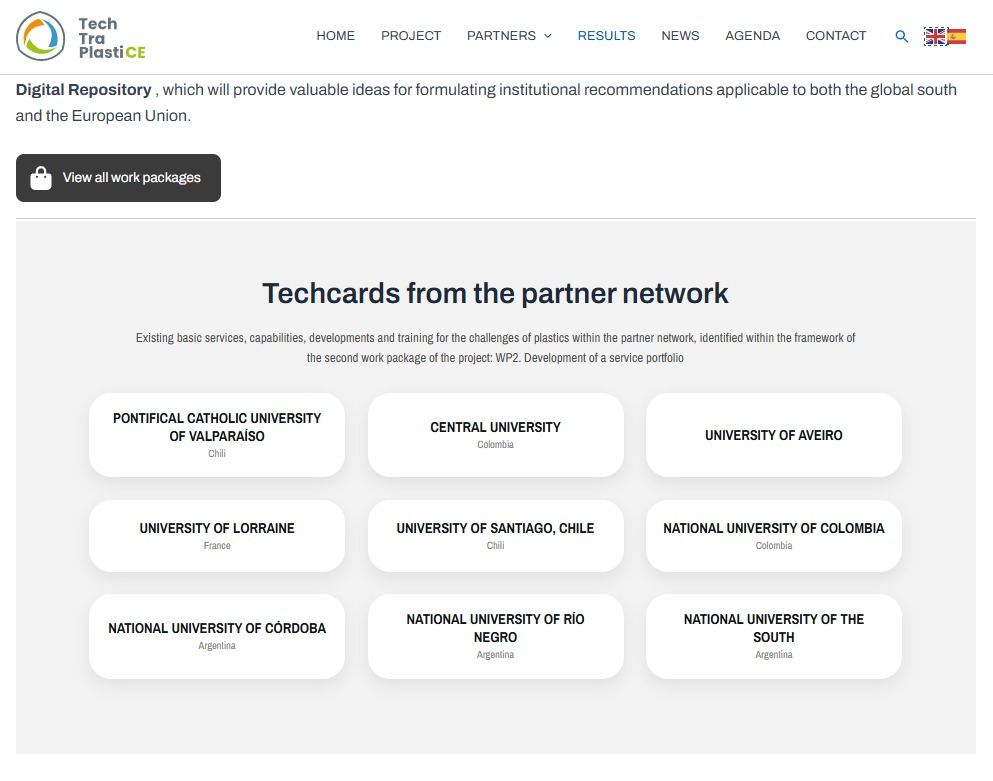
\includegraphics[width=0.8\linewidth,height=\textheight,keepaspectratio]{figures/2.2/Tech-cards-00.jpg}

}

\caption{\label{fig-techcards}Set of Tech Cards of all consortium
available on the TechTraPlastiCE website
\url{https://techtraplastice.eu/resultados/}}

\end{figure}%

Based on this material, a presentation strategy was defined to ensure
accessibility, intuitive navigation, and scalability of the system.
Initially, the possibility of organizing the repository according to the
four thematic axes was considered; however, it was ultimately structured
around the institutions, prioritizing a user-centered approach focused
on the profile of each university. Accordingly, an initial interface was
designed as the main entry point to the system, presenting a list of the
participating universities. By accessing each institution, its specific
portfolio is displayed, internally organized according to the four axes
(\emph{Training, Services, Developments, and Capabilities}). Each axis
is identified through its corresponding color code, which also functions
as a filtering criterion for the visualization of the tech cards. These
are arranged in a modular grid of four columns, with a variable number
of rows depending on the volume of information available for each
institution. This layout enables an organized, comparable, and scalable
reading experience across different levels of content.

Although the initial proposal considered the development of an
individual web page for each card, the scale of the project and the
implementation timeline led to a redefinition of this strategy. Instead,
a system based on downloadable PDF files was adopted. In this way, each
card can be viewed and downloaded directly from the interface, ensuring
its portability and independent dissemination.

The interface design was initially prototyped in Figma by the UNS team
and later shared with the UNRN team, responsible for implementing the
repository within the results section of the project's official website.
This collaborative process enabled the translation of the conceptual and
graphic guidelines defined during the design phase into a functional
solution aligned with the project's communication and accessibility
objectives.

\section{Institutional analysis (micro and meso
level)}\label{institutional-analysis-micro-and-meso-level}

Based on the analysis of the tech cards, institutional profiles were
defined for each of the participating universities. In this process,
patterns were identified in the orientation of technology transfer
activities, with particular emphasis on differences in the content of
the tech cards, the predominant types of transfer (services, development
and training), and the levels of maturity and complexity of the
identified capacities, understood as the set of resources and
competencies encompassing the various transfer mechanisms or modalities.

These capacities were also examined according to their characteristics,
which made it possible to highlight different institutional approaches
to conceptualising and implementing technology transfer. This analysis
not only enables a detailed characterisation of each institution, but
also allows for the identification of common trends and significant
differences among them. Additionally, these results were addressed from
a comparative perspective, in order to understand the diversity of
existing approaches and to identify potential complementarities among
the institutions that constitute the consortium.

\subsection{Segmentation of institutional
profiles}\label{segmentation-of-institutional-profiles}

Based on a comprehensive analysis considering the total set of tech
cards collected across all participating universities, five transfer
profiles were identified, reflecting different forms of engagement with
the environment:

\begin{itemize}
\tightlist
\item
  \textbf{Technical/technological profile}: characterised by the
  generation and application of scientific and technological knowledge
  aimed at addressing productive challenges. It includes developments,
  testing, materials characterisation and technological services, with
  varying levels of maturity.
\item
  \textbf{Social profile}: oriented towards addressing territorial,
  social and environmental challenges, with an emphasis on engagement
  with local stakeholders, sustainability and capacity building within
  the territory.
\item
  \textbf{Innovative profile}: focused on promoting innovation
  processes, including activities related to innovation management,
  business model development, organisational transfer and the
  articulation among different actors within the system.
\item
  \textbf{Educational/training profile}: focused on capacity building,
  training and knowledge dissemination through courses, workshops and
  educational activities aimed at strengthening capacities across
  different target groups.
\item
  \textbf{Hybrid profile}: characterised by a balanced combination of
  different knowledge transfer functions, integrating
  technical/technological, social, innovative and educational
  activities, without a clear predominance of any single one. This
  profile reflects a diversified institutional strategy, where
  technological services, developments, training and territory-oriented
  actions coexist, articulating multiple mechanisms of engagement with
  the environment.
\end{itemize}

This typology, developed through a comprehensive approach, also enables
the identification of recurring patterns, consistent trends and shared
criteria in transfer activities, going beyond the individual
specificities of each institution.

\section{Profile definition}\label{profile-definition}

In this section, the analysis and results for each university are
presented, considering the structure and content of their portfolios.
The approach is organised in a descriptive manner, focusing on the
content, orientation and level of advancement of technology transfer
activities, to characterise the institutional profile of each
university. Within this framework, capacities are considered as a
cross-cutting element of the analysis, as they represent the set of
institutional resources and competencies that underpin and encompass the
different types of transfer, including technical services, training and
technological developments.

The main results of the institutional analysis for each of the member
universities are presented below, based on the application of the
previously defined transfer profile typology.

\subsection{Universidad Central (UC) -
Colombia}\label{universidad-central-uc---colombia}

The profile of the Universidad Central (Figure~\ref{fig-UC}) was
analysed based on 33 technology cards, including 16 capacities forming
the knowledge and infrastructure base supporting different types of
transfer. These include 13 technical services, 3 training activities and
1 technological development.

\begin{figure}[H]

\centering{

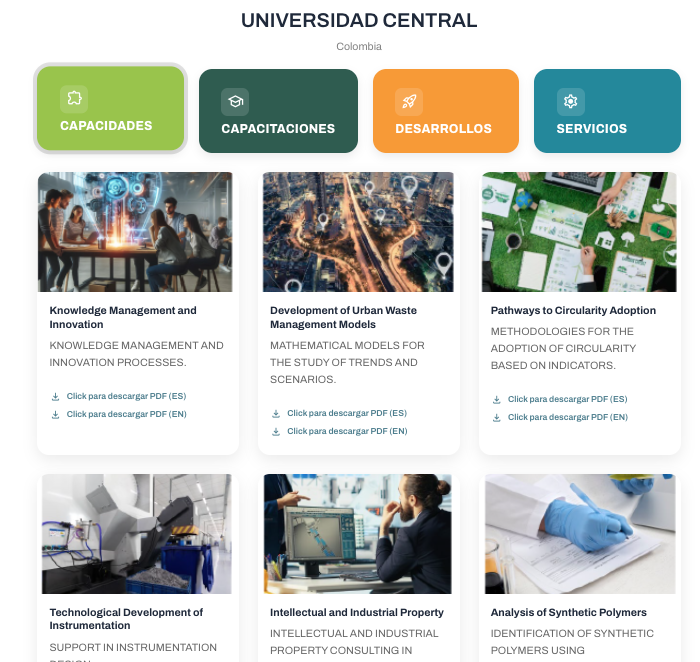
\includegraphics[width=0.6\linewidth,height=\textheight,keepaspectratio]{figures/2.2/UC.png}

}

\caption{\label{fig-UC}Tech card of the Universidad Central of Colombia.
Accessible at
\url{https://techtraplastice.eu/resultados/universidad-central/}}

\end{figure}%

The analysis shows a high relative concentration of technical services,
which constitute the core of the activities, while training and
technological developments have a significantly lower presence.
Capacities encompass both technological dimensions, such as materials
characterisation, polymer analysis, instrumentation development and
process optimisation, and organisational and management aspects,
including intellectual property, waste management models, life cycle
analysis, public policy evaluation and knowledge management. Technical
services operationalise these capacities through testing, materials
validation, prototype development, equipment maintenance, market
studies, technology watch and decision-support activities.

Transfer activities show an integrated approach, combining technological
capacities with management tools, organisational innovation and
sustainability. Compared to more strictly technological profiles, the
Universidad Central significantly incorporates components related to
circular economy, inclusion of territorial actors such as recyclers, and
public policy analysis. Based on these elements, \emph{UC can be
classified as a hybrid profile with a socio-technical orientation}.

\subsection{Universidad Nacional de Colombia
(UNAL)}\label{universidad-nacional-de-colombia-unal}

The profile of the Universidad Nacional de Colombia was analysed based
on 38 technology cards (Figure~\ref{fig-UNAL}). Within this set, 6
capacities define the institutional knowledge core. These support 22
technical services, 5 training activities and 5 technological
developments.

\begin{figure}[H]

\centering{

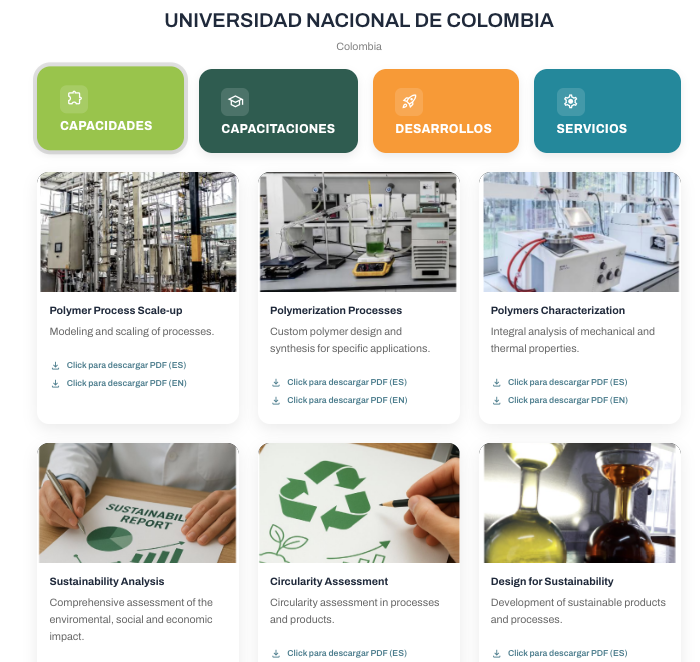
\includegraphics[width=0.6\linewidth,height=\textheight,keepaspectratio]{figures/2.2/UNAL.png}

}

\caption{\label{fig-UNAL}Tech card of the Universidad Nacional of
Colombia. Accessible at
\url{https://techtraplastice.eu/resultados/universidad-nacional-de-colombia/}}

\end{figure}%

Technical services predominate, representing more than half of the
activities, followed by training and developments. Services include a
wide range of testing and characterisation techniques for polymeric
materials, such as thermal, mechanical and physicochemical analyses,
along with advanced methodologies including chromatography,
microstructural analysis and durability assessment. Capacities also
incorporate a strategic dimension linked to sustainability, circular
economy, process scaling and materials characterisation. Training
activities reinforce this approach through courses on life cycle
analysis, eco-design and innovation. Technological developments focus on
bioeconomy and resource valorisation, including biopolymers, bio-based
plasticisers and biodegradable packaging, some reaching intermediate to
advanced maturity levels (up to TRL 7).

Transfer activities show a technological--applied orientation with a
strong environmental focus. Based on this, \emph{UNAL can be classified
within a technical/technological profile with a service-oriented and
environmental focus}.

\subsection{Pontificia Universidad Católica de Valparaíso
(PUCV)}\label{pontificia-universidad-catuxf3lica-de-valparauxedso-pucv}

Figure~\ref{fig-PUCV} presents the profile of Pontificia Universidad
Católica de Valparaíso was defined based on the analysis of a total of
31 tech cards, including: 6 technical services, 8 capacities, 8 training
activities and 9 technological developments. It is worth noting that the
identified capacities constitute the foundation upon which the different
types of transfer are articulated, integrating and supporting service,
training and development activities.

\begin{figure}[H]

\centering{

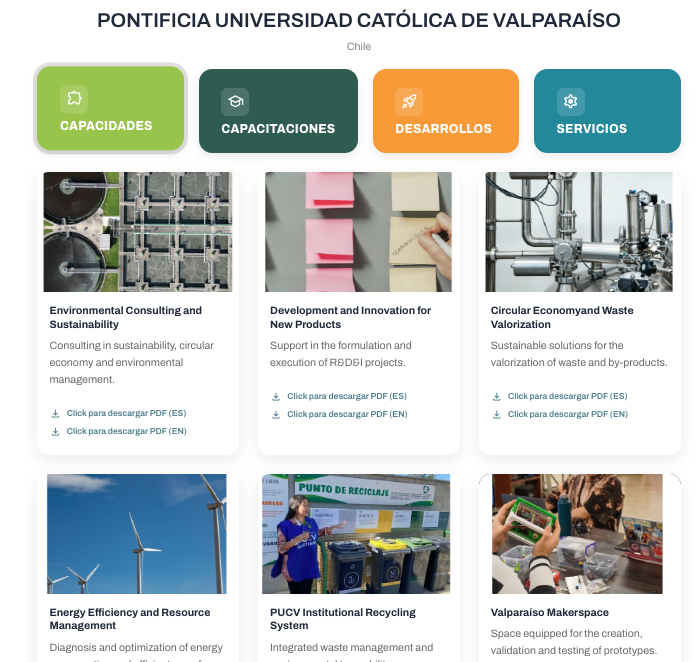
\includegraphics[width=0.6\linewidth,height=\textheight,keepaspectratio]{figures/2.2/PUCV.png}

}

\caption{\label{fig-PUCV}Tech card of the Pontificia Universidad
Católica de Valparaíso of Chile. Accessible at
\url{https://techtraplastice.eu/resultados/pontificia-universidad-catolica-de-valparaiso/}}

\end{figure}%

In terms of distribution, a relatively balanced structure is observed
across the different types of activities, with a slight predominance of
technological developments and training activities, while technical
services have a lower relative proportion. In particular, services
include laboratory testing, environmental consultancy, energy audits,
project formulation and incubation processes, while training activities
comprise diploma programmes and courses focused on innovation,
sustainability and applied technologies. Technological developments
mainly correspond to prototypes and solutions at early stages of
technological maturity (TRL 2 to 4), primarily in the fields of
materials, recycling and waste management.

The balance among activity types reflects a diversified configuration,
in which knowledge generation, service provision, training and
technological development coexist, suggesting an institutional strategy
not specialised in a single transfer mechanism. Based on these elements,
\emph{PUCV can be classified as having a hybrid profile, as it combines
different transfer functions in a balanced manner, integrating
technical, educational, innovative and engagement-oriented capacities}.

\subsection{Universidad de Santiago de Chile
(USACH)}\label{universidad-de-santiago-de-chile-usach}

The profile of the Universidad de Santiago de Chile
(Figure~\ref{fig-USACH}) was determined based on 57 tech cards (14
capacities, 24 technical services, 14 developments and 5 training
activities), indicating a diversified structure with a predominance of
services.

\begin{figure}[H]

\centering{

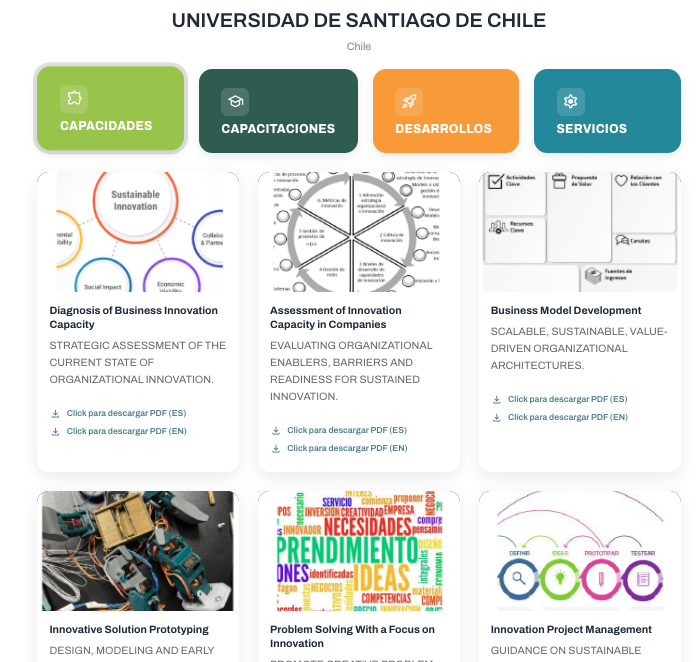
\includegraphics[width=0.5\linewidth,height=\textheight,keepaspectratio]{figures/2.2/USACH.png}

}

\caption{\label{fig-USACH}Tech card of the Universidad Santiago de
Chile. Accessible at
\url{https://techtraplastice.eu/resultados/universidad-de-santiago-de-chile/}}

\end{figure}%

Capacities focus on the development of innovation tools, organisational
management and sustainability, integrating technical and strategic
dimensions for solution design. In this sense, they function as a
conceptual and methodological support enabling the deployment of
consultancy services, company support processes and training activities,
rather than as a direct basis for highly complex technological
developments. Accordingly, technical services are primarily oriented
towards planning, optimisation and evaluation of productive and
organisational systems, incorporating modelling tools, environmental
analysis and innovation management. Technological developments cover
areas such as energy, recycled materials and circular economy, with
intermediate maturity levels (TRL 2--5). Training activities complement
the offer with courses in circular economy, innovation and agile
methodologies, supporting the adoption of these tools.

Overall, transfer activities show a hybrid orientation, combining
technological components with a strong focus on management, innovation
and sustainability. A balance is observed between services, development
and training activities, although with a lower level of technological
maturity compared to more industrially oriented profiles. Therefore,
\emph{USACH can be classified as a hybrid profile with an innovation
orientation, characterised by the articulation between management tools,
technological development and support for productive transformation
processes}.

\subsection{Universidad Nacional de Córdoba
(UNC)}\label{universidad-nacional-de-cuxf3rdoba-unc}

The profile of the Universidad Nacional de Córdoba was constructed based
on 10 technology cards, including 3 capacities, 3 technical services, 3
training activities and 1 technological development as illustrated in
Figure~\ref{fig-UNC}.

\begin{figure}[H]

\centering{

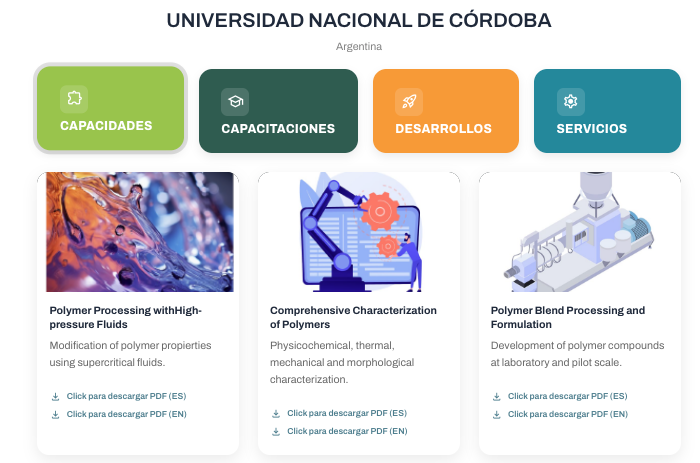
\includegraphics[width=0.6\linewidth,height=\textheight,keepaspectratio]{figures/2.2/UNC.png}

}

\caption{\label{fig-UNC}Tech card of the Universidad Nacional de Córdoba
in Argentina. Accessible at
\url{https://techtraplastice.eu/resultados/universidad-nacional-de-cordoba/}}

\end{figure}%

The portfolio shows a balanced structure between technical services and
training, with a lower presence of technological developments. However,
training activities have a relatively strong weight, indicating an
institutional orientation towards knowledge generation and dissemination
in sustainability, circular economy and emerging economic models.

Capacities are focused on polymer processing and characterisation, while
services provide support in thermal, mechanical and biodegradability
analyses. Training activities include diploma programmes and courses
with multidisciplinary approaches. A single technological development
was identified, related to biodegradable materials from cellulose at an
early maturity level (TRL 4). Based on these elements, \emph{UNC can be
classified as a hybrid profile with a technical--social orientation}.

\subsection{Universidad Nacional de Río Negro
(UNRN)}\label{universidad-nacional-de-ruxedo-negro-unrn}

The profile of the Universidad Nacional de Río Negro
(Figure~\ref{fig-UNRN}) was analysed based on 21 technology cards,
including 4 capacities, 9 technical services, 5 training activities and
3 technological developments, indicating a relatively balanced
structure.

\begin{figure}[H]

\centering{

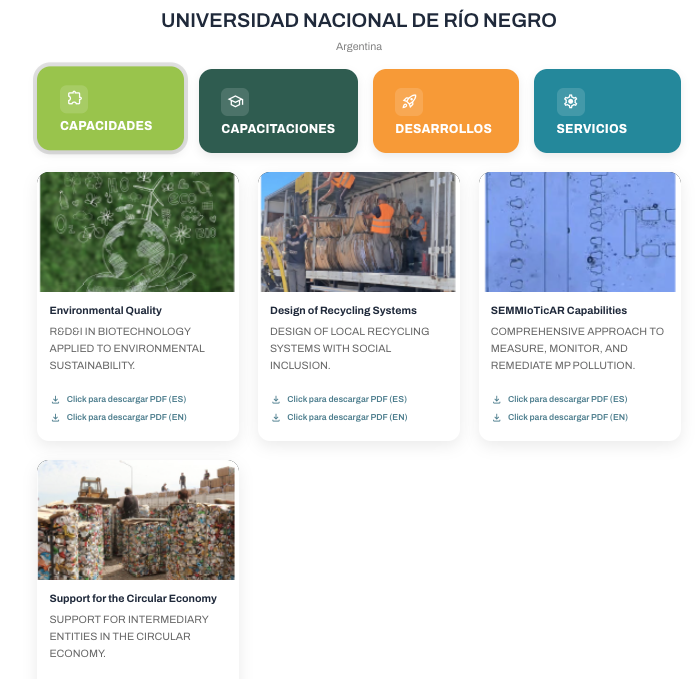
\includegraphics[width=0.5\linewidth,height=\textheight,keepaspectratio]{figures/2.2/UNRN.png}

}

\caption{\label{fig-UNRN}Tech card of the Universidad Nacional de Río
Negro in Argentina. Accessible at
\url{https://techtraplastice.eu/resultados/universidad-nacional-de-rio-negro/}}

\end{figure}%

Capacities show an integrated approach to sustainability and circular
economy, with strong emphasis on inclusive recycling systems and
interdisciplinary solutions for microplastics. These underpin technical
assistance services, training, and developments, with strong territorial
anchoring and engagement with local stakeholders and public policies.
Technical services differ from those of other institutions, focusing on
organisational consultancy, strategic planning, human resource
management and environmental diagnostics. Technological developments
address environmental challenges such as microplastic detection sensors,
microbial consortia for polymer biodegradation and environmental
management plans.

Its transfer activities show a predominantly socio-environmental
orientation with strong territorial anchoring. \emph{UNRN can be
classified within a social profile with a management and sustainability
orientation}.

\subsection{Universidad Nacional del Sur
(UNS)}\label{universidad-nacional-del-sur-uns}

The profile of the Universidad Nacional del Sur (Figure~\ref{fig-UNS})
was analysed based on 51 technology cards, including 16 capacities, 14
developments, 15 technical services and 6 training activities, showing a
highly balanced and comprehensive structure.

\begin{figure}[H]

\centering{

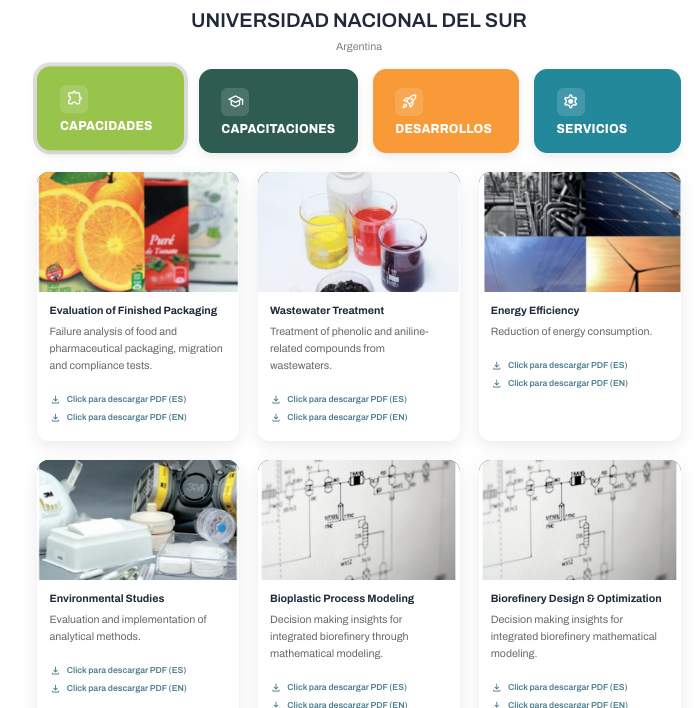
\includegraphics[width=0.6\linewidth,height=\textheight,keepaspectratio]{figures/2.2/UNS.png}

}

\caption{\label{fig-UNS}Tech card of the Universidad Nacional del Sur in
Argentina. Accessible at
\url{https://techtraplastice.eu/resultados/universidad-nacional-del-sur/}}

\end{figure}%

Capacities reflect strong expertise in process engineering, materials
science and advanced modelling, including polymer synthesis and
processing, bioplastics design, process optimisation and environmental
assessment. Technological developments are a central component, with
applications in packaging, recycling, energy and advanced materials,
spanning various maturity levels from experimental validation to
real-world implementation. Technical services are highly specialised and
supported by advanced analytical infrastructure, enabling materials
characterisation, quality control and product validation. Training
activities complement the portfolio through advanced technical
education.

The transfer activities show a clearly technological--industrial
orientation, focused on materials, processes and waste valorisation,
with strong links to the productive sector. Based on this analysis,
\emph{UNS can be classified within a technical/technological profile
with a strong orientation towards innovation and transfer}.

\subsection{Universidade de Aveiro
(UA)}\label{universidade-de-aveiro-ua}

The profile of the Universidade de Aveiro (Figure~\ref{fig-UA}) was
established based on the analysis of 29 tech cards, distributed as
follows: 12 technical services, 13 capacities, 3 training activities and
1 technological development. As with the other institutions, the
identified capacities constitute the core of the transfer offer,
concentrating technical knowledge and available infrastructure, from
which services, training activities and, to a lesser extent,
technological developments are structured and deployed.

\begin{figure}[H]

\centering{

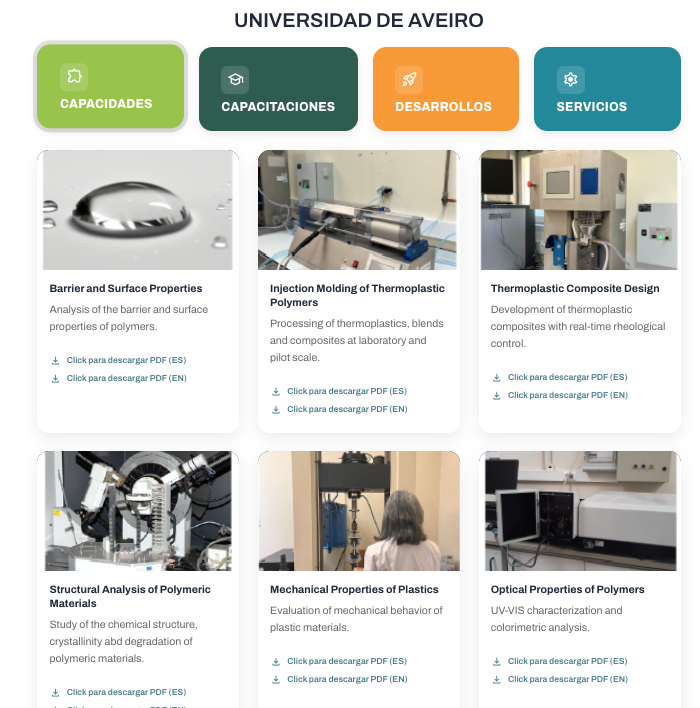
\includegraphics[width=0.6\linewidth,height=\textheight,keepaspectratio]{figures/2.2/UA.png}

}

\caption{\label{fig-UA}Tech card of the Universidade de Aveiro in
Portugal. Accessible at
\url{https://techtraplastice.eu/resultados/universidad-de-aveiro/}}

\end{figure}%

In this case, a high relative number of technical services is observed,
while training activities and, especially, technological developments
have a significantly lower proportion. Capacities are mainly oriented
towards advanced materials characterisation (mechanical, thermal,
structural, optical and morphological) and processing technologies such
as extrusion, compounding, 3D printing and injection moulding. Technical
services operationalise these capacities in applied settings, offering
testing, materials validation, process optimisation and sample
production at laboratory and pilot scale. Regarding transfer
orientation, a predominantly technological--operational approach is
evident, supported by the infrastructure available and the provision of
specialised services to the productive sector. Training activities,
although present, are focused on specific topics such as bioplastics,
sustainability and innovation, while technological developments are
limited to a single proposal with an intermediate maturity level (TRL
6), related to materials recycling.

In this context, a structure with limited diversification in transfer
mechanisms is observed, with clear specialisation in the generation of
scientific capacities and their application through technical services,
and a lower orientation towards technological development. Based on
these elements, \emph{UA can be classified within a
technical/technological profile}.

\subsection{Université de Lorraine
(UL)}\label{universituxe9-de-lorraine-ul}

The profile of the Université de Lorraine (Figure~\ref{fig-UL}) was
determined based on the analysis of 33 tech cards. Within this set, 7
capacities were identified, forming the scientific and infrastructural
basis supporting the other types of transfer. These include 17 technical
services, 7 training activities and 2 technological developments.

The composition shows a clear predominance of technical services, which
represent the main component of the identified activities, followed by
training activities, while technological developments have a more
limited presence. Technical services are primarily oriented towards
advanced characterisation of polymeric materials, including chemical,
structural, morphological, rheological and mechanical analyses, as well
as manufacturing processes, prototyping, material formulation and
specialised consultancy.

\begin{figure}[H]

\centering{

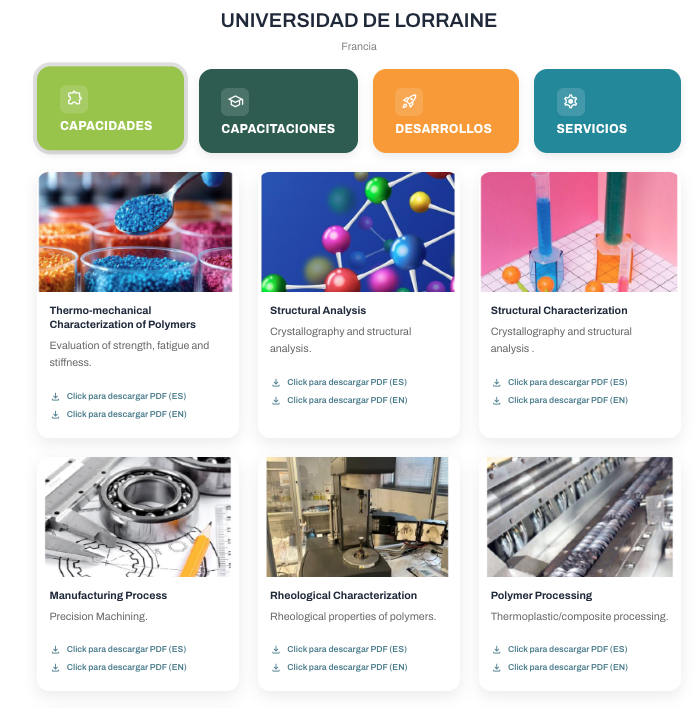
\includegraphics[width=0.6\linewidth,height=\textheight,keepaspectratio]{figures/2.2/UL.png}

}

\caption{\label{fig-UL}Tech card of the Universidade de Lorraine.
Accessible at
\url{https://techtraplastice.eu/resultados/universidaddelorraine/}}

\end{figure}%

Capacities reflect a consolidated scientific infrastructure focused on
polymer characterisation and processing, with emphasis on understanding
structure--property--process relationships. Training activities
complement this framework through a broad and structured educational
offer, ranging from specialised short courses to full engineering
programmes, showing strong integration between academic training and
applied research. Regarding transfer orientation, a strongly
scientific--technological approach is observed, based on the generation
of advanced knowledge and its application through highly specialised
services. Technological developments are positioned at intermediate
maturity levels (TRL 4), indicating a focus on experimental validation
and proof of concept.

The structure is relatively diversified but clearly specialised in
high-level technical services, strongly supported by scientific
capacities and a consolidated training offer. \emph{Based on these
elements, UL can be classified within a technical/technological
profile.}

\section{Comparative analysis of the profiles of each university (macro
level) and definition of the consortium
profile}\label{comparative-analysis-of-the-profiles-of-each-university-macro-level-and-definition-of-the-consortium-profile}

The macro-level analysis focused on the aggregation and characterisation
of the institutional portfolios of the participating universities, based
on the set of tech cards collected in each case. This approach made it
possible to identify patterns in the structure, orientation and level of
development of transfer activities, as well as differences in
institutional strategies for engagement with the environment. Within
this framework, capacities are recognised as the structuring element of
the portfolios, as they concentrate the knowledge, infrastructure and
institutional competencies from which technical services, training
activities and technological developments originate and are deployed.
Thus, the differences observed among institutions largely reflect the
nature, scope and orientation of these capacities.

In general terms, a high degree of heterogeneity is observed in the
composition of the portfolios, both in the distribution across activity
types and in the level of technological maturity. Nevertheless, three
main institutional configurations can be identified. On the one hand,
there are institutions with a technical/technological profile, where
capacities are strongly anchored in scientific and experimental
capabilities supported by advanced infrastructure. In these cases,
technical services constitute the main transfer mechanism,
operationalising these capacities through testing, materials
characterisation and support to industrial processes, while
technological developments complement this with varying levels of
maturity. Secondly, institutions with a social orientation are
identified, where capacities are structured around environmental, social
and sustainability-related challenges. In these contexts, services take
the form of technical assistance, consultancy and support to territorial
actors, while training activities play a central role in local capacity
building and technological developments are oriented towards
context-specific solutions. Finally, institutions with hybrid profiles
are identified, characterised by a balanced configuration between
services, developments and training. In these cases, capacities act as
an integrative support, enabling both service provision and the
development of technological solutions and management tools, combining
technical, organisational and innovation components.

In addition, the analysis of institutional profiles allowed the
identification of patterns across two key dimensions: on the one hand,
the orientation of transfer, which ranges from technological--industrial
approaches to socio-territorial ones; and, on the other hand, the level
of development of transfer activities, linked to the degree of
consolidation of capacities and their deployment in services and
technological developments. This approach contributes to a deeper
understanding of the differences among institutions and enriches the
interpretation of the identified profiles. Furthermore, the analysis of
technological maturity levels reveals significant differences among
institutions, ranging from early-stage validation developments to
technologies implemented in real environments, reflecting different
degrees of consolidation of transfer systems.

In order to synthesise these differences, the matrix presented in
Figure~\ref{fig-comp} was developed, allowing the relative positioning
of universities to be represented based on two dimensions: the
orientation of transfer and the level of advancement of the transfer
offer. The first dimension, represented on the horizontal axis,
expresses a continuum ranging from socio-territorial approaches, focused
on engagement with local actors, sustainability and capacity building in
the territory, to technological approaches oriented towards the
development of applied solutions and engagement with the productive
sector. The vertical axis reflects the quantity and level of advancement
of the transfer offer, considering both the degree of development and
consolidation of institutional capacities and the technological maturity
of developments.

\begin{figure}[H]

\centering{

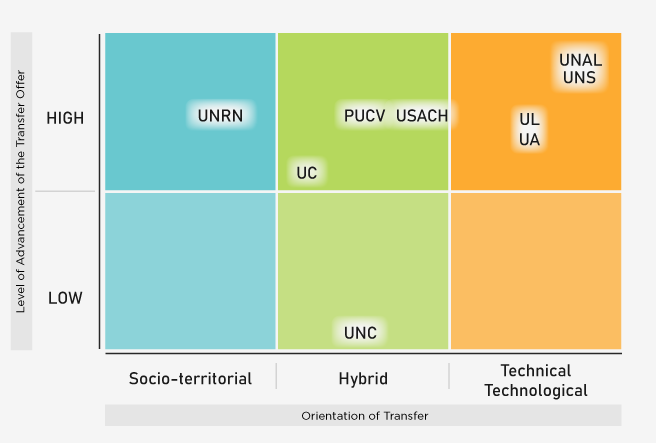
\includegraphics[width=0.85\linewidth,height=\textheight,keepaspectratio]{figures/2.2/6.png}

}

\caption{\label{fig-comp}Comparative matrix of transfer offer.}

\end{figure}%

As expected, based on the previous analyses, the matrix allows the
visualisation of differences among universities and highlights the
coexistence of multiple transfer strategies. It also reflects different
levels of maturity, consolidation and institutional orientations of the
transfer offer, contributing to a more comprehensive understanding of
the diversity of profiles within the consortium. Furthermore, by
incorporating a comparative perspective by country and region,
additional trends are identified that reinforce and complement the
institutional analysis.

In Colombia (Universidad Central and Universidad Nacional de Colombia),
an articulation between technological capacities and approaches oriented
towards sustainability and the circular economy is observed, with a
strong presence of technical services. However, differences in
orientation can be identified: while UNAL presents a more technological
profile, Universidad Central places greater emphasis on
socio-territorial and management dimensions, resulting in hybrid
profiles with different levels of development.

In Chile (PUCV and USACH), portfolios are characterised by
diversification and a significant presence of services and training
activities, accompanied by technological developments at intermediate
maturity stages. Capacities are mainly oriented towards innovation,
sustainability and management, leading to hybrid profiles with an
emphasis on engagement with the productive sector and support to
innovation processes.

In Argentina (UNS, UNC and UNRN), greater institutional heterogeneity is
observed. UNS presents a consolidated technical/technological profile,
with strong integration between capacities, services and developments at
different maturity levels. In contrast, UNRN shows a social profile,
with strong anchoring in sustainability and engagement with local
actors. UNC is positioned in an intermediate point, with a hybrid
profile and a technical--social orientation.

Finally, in Europe (Université de Lorraine and Universidade de Aveiro),
technical/technological profiles predominate, with a strong emphasis on
consolidated scientific capacities and the provision of specialised
technical services. In these cases, transfer is primarily structured
around advanced infrastructure and experimental knowledge, with a lower
relative weight of technological developments and a clear orientation
towards industrial support.

The macro-level analysis shows that, although all institutions deploy
multiple transfer mechanisms, there are dominant logics associated with
their capacities that shape differentiated profiles according to their
orientation, level of development and institutional context. This level
is key to understanding the identity of each university in terms of
transfer and its relative positioning within the consortium, as well as
to identifying opportunities for articulation and complementarities.

\chapter{Conclusions}\label{conclusions}

This deliverable represents a key step in transforming the initial
dataset collected in D2.1 into structured, validated, and actionable
knowledge within the framework of the TechTraPlastiCE project. Through a
systematic process of data review, validation, and standardization, the
information provided by partner institutions was consolidated into a
coherent and comparable dataset, ensuring its reliability and analytical
robustness. The development of tech cards as standardized units enabled
the organization of diverse institutional capacities into a consistent
format, facilitating both analysis and communication. Building upon
this, institutional portfolios were constructed, moving beyond a simple
inventory of activities towards structured representations of each
university's potential contribution to the plastic circular economy.

The multi-level methodological approach (micro, meso, and macro) allowed
not only the detailed characterization of individual capacities and
institutional profiles but also the identification of broader patterns,
complementarities, and strategic opportunities across the consortium.
This analysis highlighted the diversity of transfer approaches, ranging
from technical/technological to socio-territorial orientations, as well
as hybrid configurations that integrate multiple functions. Overall, the
results demonstrate that higher education institutions play a critical
role as enablers of the circular economy for plastics, with
differentiated but complementary capacities. By structuring these
capacities into accessible and strategic service portfolios, this
deliverable strengthens the ability of universities to engage with
external stakeholders, respond to real-world challenges, and generate
impact at both regional and international levels.


\backmatter


\end{document}
